% \iffalse meta-comment
% vim: textwidth=75
%<*internal>
\iffalse
%</internal>
%<*readme>

--------:| ----------------------------------------------------------------
schemata:| Generic package to aid construction of topical categories
  Author:| Charles P. Schaum
  E-mail:| charles dot schaum@comcast.net
 License:| Released under the LaTeX Project Public License v1.3c or later
     See:| http://www.latex-project.org/lppl.txt

Short description:
The schemata package helps the creation of topical outlines that illustrate the breakdown of concepts and categories in academic texts from the late medieval to early modern periods.

Files		    Distribution

README        This file
schemata.pdf  Documentation
schematest.tex  Test file for Plain TeX or Eplain
schemata.png  Image file used for the manual

Makefile      Automates building with GNU make 3.81
schemata.dtx  Documented LaTeX file containing both code and documentation

Installation

Download the package from

https://www.ctan.org/tex-archive/macros/generic/schemata

Unpack schemata.zip in an appropriate directory.

If you have a make utility compatible with GNU make, either in
GNU/Linux, a BSD variant, OSX, or Cygwin in Windows you can type

	make inst

to install the package into your $TEXMFHOME tree or

	make install

to install the package into your $TEXMFLOCAL tree for all users.
The latter requires sudo privileges.

Other useful targets include:

	(release process)

	make release			The default target, same as just ``make''.

	make clean				Removes all intermediate files. Left are
							the files listed above plus schemata.sty.

	make distclean			Leave only schemata.dtx, schematest.tex,
							schemata.png, and Makefile.

	make zip				Generate a zip file ready for distribution.

	(testing process)

	make testing			Release files, plus compiles schematest.tex.

It is not necessary, however, to use GNU make. One can generate
the package files manually. Since the files schemata.ins and README.txt
are contained in the .dtx file itself, the first step is to generate
the installer driver schemata.ins, plus the file README.txt, which will
also trigger the extraction of schemata.sty and produce the first pass of
the package documentation schemata.pdf:

	pdflatex -shell-escape -recorder -interaction=batchmode schemata.dtx

Next one adds a table of contents and all cross-references, this also
should finalize page numbers for glossary and index input files:

	pdflatex --recorder --interaction=nonstopmode schemata.dtx
	
The next commands generate the glossary/index output files:
	
	makeindex -q -s gglo.ist -o schemata.gls schemata.glo
	makeindex -q -s gind.ist -o schemata.ind schemata.idx
	
The final two commands integrate the glossary (changes) and index:
	
	pdflatex --recorder --interaction=nonstopmode schemata.dtx
	pdflatex --recorder --interaction=nonstopmode schemata.dtx

Now one can either keep README.txt or rename it to README, e.g.:

	mv README.txt README

Normally one creates the following directories for a user:

	$TEXMFHOME/source/generic/schemata		dtx file, schemata.png
	$TEXMFHOME/doc/generic/schemata			pdf file, README, schematest.tex,
	                                       
		
and creates the following directories for the local site:

	$TEXMFLOCAL/source/generic/schemata		dtx file, schemata.png
	$TEXMFLOCAL/doc/generic/schemata		pdf file, README, schematest.tex,
	                                       

The above environment variables often are /usr/local/texlive/texmf-local for
$TEXMFLOCAL and ~/texmf for $TEXMFHOME.

The make process normally renames the README.txt file created from the
dtx file to just README by using mv (move / rename utility in the *nix
userland). Windows distributions of TeX and LaTeX often keep the txt file
because of using file extensions instead of ``magic numbers'' to identify
files.

Run mktexlsr with the appropriate level of permissions to complete the
install.

This packages works with LaTeX and Plain TeX.

License

This material is subject to the LaTeX Project Public License:
http://www.ctan.org/tex-archive/help/Catalogue/licenses.lppl.html

Happy TeXing!
%</readme>
%<*internal>
\fi
\def\nameofplainTeX{plain}
\ifx\fmtname\nameofplainTeX\else
  \expandafter\begingroup
\fi
%</internal>
%<*install>
\input docstrip.tex
\keepsilent
\askforoverwritefalse
\preamble

--------:| ----------------------------------------------------------------
schemata:| Generic package to aid construction of topical categories
  Author:| Charles P. Schaum
  E-mail:| charles dot schaum@comcast.net
 License:| Released under the LaTeX Project Public License v1.3c or later
     See:| http://www.latex-project.org/lppl.txt

\endpreamble
\postamble

Copyright (C) 2020 by Charles P. Schaum <charles dot schaum@comcast.net>

This work may be distributed and/or modified under the
conditions of the LaTeX Project Public License (LPPL), either
version 1.3c of this license or (at your option) any later
version.  The latest version of this license is in the file:

http://www.latex-project.org/lppl.txt

This work is "maintained" (as per LPPL maintenance status) by
Charles P. Schaum.

This work consists of the file schemata.dtx, schematest.tex,
  schemata.png, and a Makefile.
Running "make" generates the derived files README, schemata.pdf,
  and schemata.sty.
Running "make inst" installs the files in the user's TeX tree.
Running "make install" installs the files in the local TeX tree.

\endpostamble

\usedir{tex/generic/schemata}
\generate{
  \file{\jobname.sty}{\from{\jobname.dtx}{package}}
}
%</install>
%<install>\endbatchfile
%<*internal>
\usedir{source/generic/schemata}
\generate{
  \file{\jobname.ins}{\from{\jobname.dtx}{install}}
}
\nopreamble\nopostamble
\usedir{doc/generic/schemata}
\generate{
  \file{README.txt}{\from{\jobname.dtx}{readme}}
}
\ifx\fmtname\nameofplainTeX
  \expandafter\endbatchfile
\else
  \expandafter\endgroup
\fi
%</internal>
% \fi
%
% \iffalse
%<*driver>
\ProvidesFile{schemata.dtx}
%</driver>
%<package>{\expandafter}\expandafter\ifx \csname schemataLaTeX\endcsname\relax
%<package>  \def\schemataLaTeX{LaTeX2e}\fi
%<package>\ifx\fmtname\schemataLaTeX
%<package>\expandafter\NeedsTeXFormat\expandafter{\schemataLaTeX}
%<package>\ProvidesPackage{schemata}
%<*package>
  [2020/03/14 v1.1 generic package to aid construction of topical categories]
%</package>
%<package>\fi
%<*driver>
\documentclass[11pt]{ltxdoc}
\usepackage[T1]{fontenc}
\usepackage[polutonikogreek,american]{babel}
\newcommand{\gk}[1]{\foreignlanguage{polutonikogreek}{#1}}
\usepackage{lmodern}
\usepackage[textwidth=140mm,textheight=237mm,right=25mm,nohead]{geometry}
\usepackage{graphicx}
%^^A Dangerous bend ahead...
\usepackage{manfnt}
%^^A Use the MetaPost logo
\usepackage{mflogo}
\usepackage[toc]{multitoc}
\usepackage{paracol}
\usepackage{\jobname}
\usepackage{verbatim}
\usepackage[numbered]{hypdoc}

%^^A Let verbatim environments be numbered or unnumbered, and start or resume that.
\makeatletter
\newcommand*\ClearNum{%^^A
  \newcounter{VerbLine}\setcounter{VerbLine}{0}%^^A
  \def\verbatim@processline{\expandafter\@gobble\the\verbatim@line\par}%^^A
}
\newcommand*\StartNum{%^^A
  \setcounter{VerbLine}{0}
  \def\verbatim@processline{\stepcounter{VerbLine}\leavevmode%^^A
  \llap{\footnotesize\normalfont\theVerbLine\quad}%^^A
  \expandafter\@gobble\the\verbatim@line\par}%^^A
}
\newcommand*\ContinueNum{%^^A
  \def\verbatim@processline{\stepcounter{VerbLine}\leavevmode%^^A
  \llap{\footnotesize\normalfont\theVerbLine\quad}%^^A
  \expandafter\@gobble\the\verbatim@line\par}%^^A
}
\makeatother
%^^A Set up numbered verbatim
\ClearNum

%^^A Macros for marginalia.
\newcommand*\Version[1]{\unless\ifinner\marginpar{\strut\raggedleft\textsf{\bfseries#1}}\fi}
\newcommand*\VersionWarn[1]{{\unless\ifinner\marginpar{\strut\raggedleft\textsf{\bfseries#1}\break\small\dbend}\fi}}
\newcommand*\Warn{{\unless\ifinner\marginpar{\strut\small\raggedleft\dbend}\fi}}
\newcommand*\Info[1]{{\unless\ifinner\marginpar{\strut\small\raggedleft#1}\fi}}

%^^A Struts for framed boxes
\newcommand*{\mystrut}{\rule[-0.25\baselineskip]{0pt}{\baselineskip}}

\EnableCrossrefs
\CodelineIndex
\RecordChanges
\begin{document}
  \DocInput{\jobname.dtx}
\end{document}
%</driver>
% \fi
%
% \CheckSum{594}
%
% \CharacterTable
%  {Upper-case    \A\B\C\D\E\F\G\H\I\J\K\L\M\N\O\P\Q\R\S\T\U\V\W\X\Y\Z
%   Lower-case    \a\b\c\d\e\f\g\h\i\j\k\l\m\n\o\p\q\r\s\t\u\v\w\x\y\z
%   Digits        \0\1\2\3\4\5\6\7\8\9
%   Exclamation   \!     Double quote  \"     Hash (number) \#
%   Dollar        \$     Percent       \%     Ampersand     \&
%   Acute accent  \'     Left paren    \(     Right paren   \)
%   Asterisk      \*     Plus          \+     Comma         \,
%   Minus         \-     Point         \.     Solidus       \/
%   Colon         \:     Semicolon     \;     Less than     \<
%   Equals        \=     Greater than  \>     Question mark \?
%   Commercial at \@     Left bracket  \[     Backslash     \\
%   Right bracket \]     Circumflex    \^     Underscore    \_
%   Grave accent  \`     Left brace    \{     Vertical bar  \|
%   Right brace   \}     Tilde         \~}
%
%
% \changes{v0.5}{2013/02/14}{Initial version}
% \changes{v0.6}{2013/03/10}{Added features}
% \changes{v0.7}{2013/09/23}{Changed contact info}
% \changes{v0.8}{2016/01/25}{Rewrote manual; moved to dtxgen}
% \changes{v1.1}{2020/03/14}{Fix issue with dtx guards}
%
% \GetFileInfo{\jobname.dtx}
% \DoNotIndex{\bgroup, \csname, \DeclareOption, \def, \dimen, \egroup, \else, \endcsname, \endinput, \ExecuteOptions, \expandafter, \fi, \futurelet, \gdef, \hbox, \hfil, \if, \ifcsname, \ifdim, \ifmmode, \ifx, \ignorespaces, \index, \let, \newbox, \newcommand, \newdimen, \newif, \next, \PackageWarning, \ProcessOptions, \relax, \RequirePackage, \setbox, \space, \testchar, \vbox, \vcenter, \vfil, \vskip}
%
%\title{\textsf{schemata} --- Generic package to aid construction of topical categories\thanks{This file
%   describes version \fileversion, last revised \filedate.}
%}
%\author{Charles P. Schaum\thanks{E-mail: charles dot schaum@comcast.net}}
%\date{Released \filedate}
%
%\maketitle
%
% \begin{abstract}
% \noindent The \textsf{schemata} package helps the creation of topical outlines that illustrate the breakdown of concepts and categories in academic texts from the late medieval to early modern periods.
% \end{abstract}
%
% \tableofcontents
%
% \section{Introduction}
%
% This package uses boxes and math mode to typeset \emph{schemata} (plural of \gk{t'o sq~hma} or \emph{schema}, meaning \emph{form}, \emph{shape}, \emph{appearance}, etc.). One sees them in academic literature from at least the seventeenth through the nineteenth centuries.\footnote{Books that use this package include: Löhe, \textit{The Pastor} [\textit{Der evangelische Geistliche}] (St.~Louis, 2015) and Schaum and Coll\-ver, \textit{Breath of God, Yet Work of Man} (St.~Louis, 2019).}
%
% Packages like \emph{TikZ}, \textsf{PSTricks}, \MP, or other solutions have advantages over this one, especially for those seeking a top-to-bottom diagram.\footnote{For example: \textsc{H.~Dembowski}, \emph{Einf{\"u}hrung in die Christologie} (Darmstadt, 1993), 146.}
% Yet these packages may present challenges if one has to implement both open \emph{and} closed braces in a schema, which math mode allows.
% \newpage
%
% \section{Usage}
%
% \subsection[Loading and Options]{Package Loading and Options}
%
% The \textsf{schemata} package is a minimal ``wrapper'' for math mode. It can be used with \LaTeX{} or with several generic formats, such as \PlainTeX{} and Eplain, even Lollipop, but not \textsc{Con\TeX t}:\footnote{It appears that \textsc{Con\TeX t} does not like nesting math-mode expressions within boxes in the manner used by this package. Barring a rewrite of \textsf{schemata}, that is the \emph{status controversiae}.}
% \begin{quote}
% \fbox{\begin{tabular}{ll}
% {\Large\strut}For \LaTeX{} invoke: & \cmd{\usepackage}\oarg{options}\texttt{\{schemata\}}\\
% {\Large\strut}For generic use: & \cmd{\input}\texttt{\textvisiblespace schemata.sty}
% \end{tabular}}
% \end{quote}\smallskip
% 
% \DescribeMacro{\schemataLaTeX}
% Normally, \textsf{schemata} uses generic \TeX{} macros if the format is not \LaTeXe. When using a \LaTeX-like format with a different name than \texttt{LaTeX2e}, one theoretically could insert the following before |\usepackage{schemata}|:
% \begin{quote}
% |\edef\schemataLaTeX{\fmtname}|
% \end{quote}
% 
% Yet\Warn{} this is usually unneeded. We want \cmd{\schemataLaTeX} to be undefined before \texttt{schemata.sty} is loaded to get the default value \texttt{LaTeX2e}. We recommend not using this macro unless you know what you are doing.\medskip
% 
% \LaTeX\Info{options} users can choose one among four package options: \texttt{braces}, \texttt{brackets}, \texttt{parens}, and \texttt{groups}. These set the defaults for the delimiters. If no options are chosen, the default is \texttt{braces}.
% 
% \subsection{Macro Overview}
%
% One can describe schemata as a grouping of boxes that contain content, whose relationships are demonstrated by delimiters. We start with the boxes and their content. Subsequently, we deal with the delimiters, then later, the manner of grouping and arrangement, as well as tweaks and tutorials.
% 
% \subsubsection[\texttt{\textbackslash schemabox}]{Containers: \texttt{\textbackslash schemabox}}
% 
% \DescribeMacro{\schemabox}
% Schemata contain vertically-centered lists of material in inner vertical mode. When in a \cmd{\schema} or a \cmd{\Schema} (see below), a \cmd{\schemabox} stacks one or more lines of \cmd{\hbox}-enclosed text in a \cmd{\vbox.} It redefines the macro |\\| to close the current \cmd{\hbox} and begin a new one, with some options that can be modified (Section~\ref{sec:tweakschema}).
% \begin{quote}
% \fbox{\begin{tabular}{l}
% {\Large\strut}\cmd{\schemabox}\oarg{width}\marg{text}\\
% \end{tabular}}
% \end{quote}
% The \meta{width} of a \cmd{\schemabox} is a dimension, e.g., \texttt{3cm}. No text wrapping (as in a \cmd{\parbox}) takes place. If there is more than one line of text, each line of \meta{text} must be terminated explicitly by |\\|, except the final line. Usually, the first line of a \cmd{\schemabox} inserts a \cmd{\strut} for aesthetic reasons.
%
% When not in internal vertical mode, \cmd{\schemabox} ignores \meta{width}, does not redefine |\\|, and prints its argument as text: |\schemabox{line~1\\ line~2}| \schemabox{line~1\\ line~2}. This helps prevent errors.
% \newpage
%
% \subsubsection{Delimiters}
% 
% \DescribeMacro{\DoBraces}
% Both generic \TeX{} and \LaTeX{} users can use these four macros to set or change the type of delimiters.
% \DescribeMacro{\DoBrackets}
% In both generic \TeX{} and \LaTeX, the default delimiter is braces.
% \DescribeMacro{\DoParens}
% \cmd{\DoBraces}, \cmd{\DoBrackets}, \cmd{\DoParens}, and \cmd{\DoGroups} do the same thing as the respective package options,
% \DescribeMacro{\DoGroups}
% except they also change the delimiters when used before \cmd{\schema} and \cmd{\Schema}. They remain in force until the end of a scope:\label{page:SBNudge}
% \begin{displaymath}
% \DoBrackets\bgroup\renewcommand\SBNudgeFactor{\kern0.08em}
% \Schema{0ex}{2.3ex}{\schemabox{a}}{\Schema[close]{0ex}{2.4ex}{\NudgeSB\schemabox{b\\c}}{\schemabox{d}}}\egroup
% \qquad\DoParens
% \Schema{0ex}{2.3ex}{\schemabox{a}}{\Schema[close]{0ex}{2.4ex}{\schemabox{b\\c}}{\schemabox{d}}}
% \qquad\DoGroups
% \Schema{0ex}{2.3ex}{\schemabox{a}}{\Schema[close]{0ex}{2.4ex}{\schemabox{b\\c}}{\schemabox{d}}}
% \qquad\DoBraces
% \Schema{0ex}{2.3ex}{\schemabox{a}}{\Schema[close]{0ex}{2.4ex}{\schemabox{b\\c}}{\schemabox{d}}}
% \end{displaymath}
%
% Additionally, these macros can change the delimiter style within a schema. See Section~\ref{sec:multiple}, as well as the example below:\bigskip
% 
% \leavevmode\quad\begin{minipage}[c]{0.6\textwidth}\small
% \StartNum
% \begin{verbatim}
%\DoBrackets
%\Schema{0ex}{2.4ex}
%  {\schemabox{a}}
%  {\DoParens\Schema[close]{0ex}{2.3ex}
%    {\schemabox{b\\c}}
%    {\schemabox{d}}
%}\end{verbatim}
% \end{minipage}
% \begin{minipage}[c]{0.25\textwidth}
% \begin{displaymath}
% \DoBrackets\Schema{0ex}{2.4ex}
%   {\schemabox{a}}
%   {\DoParens\Schema[close]{0ex}{2.3ex}
%     {\schemabox{b\\c}}
%     {\schemabox{d}}}
% \end{displaymath}\medskip
% \end{minipage}\bigskip
% 
% One can add new types by using eligible math-mode delimiters, e.g.:\bigskip
% 
% \leavevmode\quad\begin{minipage}[c]{0.6\textwidth}\small
% \StartNum
% \begin{verbatim}
%\makeatletter
%\newcommand*{\DoVerts}%
%  {\let\@schemata@LD\bracevert%
%   \let\@schemata@RD\bracevert}
%\makeatother
%\DoVerts
%\Schema{0ex}{5ex}
%  {\vskip0.6ex\schemabox{a}}
%  {\Schema[close]{0ex}{5ex}
%    {\vskip0.4ex\schemabox{b\\c\\d\\e}}
%    {\vskip0.6ex\schemabox{{\kern0.1em}f}}
%}\end{verbatim}
% \end{minipage}
% \begin{minipage}[c]{0.25\textwidth}
% \makeatletter
% \newcommand*{\DoVerts}%
%   {\let\@schemata@LD\bracevert%
%    \let\@schemata@RD\bracevert}
% \makeatother
% \DoVerts
% \begin{displaymath}
% \Schema{0ex}{5ex}
%   {\vskip0.6ex\schemabox{a}}
%   {\Schema[close]{0ex}{5ex}
%     {\vskip0.4ex\schemabox{b\\c\\d\\e}}
%     {\vskip0.6ex\schemabox{{\kern0.1em}f}}
% }
% \end{displaymath}\medskip
% \end{minipage}
%
% \subsubsection[\texttt{\textbackslash schema}]{Leaf Nodes: \texttt{\textbackslash schema}}
%
% \DescribeMacro{\schema}
% A ``simple'' schema has a left-hand side with vertically-centered vertical material, a brace, and a right-hand side with vertically-centered vertical material:
% \begin{quote}
% \fbox{\begin{tabular}{l}
% {\Large\strut}\cmd{\schema}\oarg{type}\marg{left side}\marg{right side}\\
% \end{tabular}}
% \end{quote}
% The \meta{left side} and \meta{right side} are vertical material in order to allow a \cmd{\smallskip} or other vertical adjustment as needed.\medskip
% 
% The \meta{type} of a schema is \texttt{open} (the delimiter opens to the right) by default:
% 
% \leavevmode\quad\begin{minipage}[c]{0.6\textwidth}\small
% \StartNum
% \begin{verbatim}
%\schema
%  {\schemabox{a}}
%  {\schemabox{b\\c}}\end{verbatim}
% \end{minipage}
% \begin{minipage}[c]{0.25\textwidth}
% \begin{displaymath}
% \schema
%   {\schemabox{a}}
%   {\schemabox{b\\c}}
% \end{displaymath}\vspace{0pt}
% \end{minipage}
% \newpage
% 
% Any value of \meta{type} other than the exact string \texttt{open} makes a ``closed'' schema (the delimiter opens to the left):
%
% \leavevmode\quad\begin{minipage}[c]{0.6\textwidth}\small
% \StartNum
% \begin{verbatim}
%\schema[closed]
%  {\NudgeSB\schemabox{b\\c}}
%  {\schemabox{a}}\end{verbatim}
% \end{minipage}
% \begin{minipage}[c]{0.25\textwidth}
% \begin{displaymath}
% \schema[closed]
%   {\NudgeSB\schemabox{b\\c}}
%   {\schemabox{a}}
% \end{displaymath}\vspace{0pt}
% \end{minipage}
% 
% Using \cmd{\NudgeSB} above added a kern of \texttt{0.2em} at the right of the \cmd{\schemabox} to offset an automatic kern of \texttt{-0.2em} that normally pulls the brace slightly closer to the left-hand side when it opens to the right. We cover such tweaks in Section~\ref{sec:tweakschema}.
% 
% In practice, \cmd{\schema} does not nest, so it is only useful for the right-hand ``leaves'' of a large schema. That makes formatting the ``leaves'' much faster. Thus, the \cmd{\schema} macro is used only in the framed sub-schemata below.\smallskip
%
% \noindent\leavevmode\begin{minipage}[c]{0.6\textwidth}
% \quad\space The automatic sizing of \cmd{\schema} changes, depending on the height, depth, and even context of the letters. This can look ugly if uniformity is desired. Use \cmd{\Schema} (next section) to enforce uniform schemata. Section~\ref{sec:tweakschema} gives more details on tweaking \cmd{\schema} as needed.
% \end{minipage}\hfill
% \begin{minipage}[c]{0.235\textwidth}\small
%   \Schema{-1ex}{4.2ex}
%     {
%       \schemabox{a}
%     }
%     {
%       \vbox{\noindent%
%         \fbox{\schema{\schemabox{b}}{\SwitchSB\schemabox{c\\d}}}\\[1ex]
%         \fbox{\schema{\schemabox{e}}{\schemabox{f\\g}}
%       }
%     }
%   }
% \end{minipage}
%
% \subsubsection[\texttt{\textbackslash Schema}]{Branches and Root: \texttt{\textbackslash Schema}}
%
% \DescribeMacro{\Schema}
% The ``complex'' form of a schema also has a left-hand side with vertically-centered vertical material, a brace, and a right-hand side of vertically-centered vertical material, along with two arguments that adjust the layout:
% \begin{quote}
% \fbox{\begin{tabular}{l}
% {\Large\strut}\cmd{\Schema}\oarg{type}\marg{adjust}\marg{size}\marg{left side}\marg{right side}\\
% \end{tabular}}
% \end{quote}
%The \meta{type} is |open| by default. As above, any other \meta{type} except the exact string |open| will make it a ``closed'' schema. Both \meta{adjust} and \meta{size} are dimensions. We recommend expressing them as \texttt{ex}. This allows for easier scaling of the schema when changing the font size. Here is how to set \meta{adjust}:\footnote{Instead of setting \meta{adjust}, one could put vertical skips either before or after \cmd{\schemabox}, \cmd{\schema}, or \cmd{\Schema}. Yet using braces as delimiters tends to draw material toward the center cusp, where \meta{adjust} keeps that centered look while allowing some adjustments.}
% \begin{quote}
% \begin{tabular}{lll}
% \textbf{negative} & left side and delimiter up & right side down\\[0.5ex]
% \textbf{positive} & left side and delimiter down & right side up\\
% \end{tabular}
% \end{quote}
%
% Set the delimiter \meta{size} to be a scaled value of ex just a bit larger than the number of lines of text that the delimiter spans.
%
% By using \cmd{\Schema} to adjust the delimiter height and centering, one can bypass the shortcomings of \cmd{\schema}, but at the cost of time. One has to traverse the schema at least twice to get the desired layout. \cmd{\Schema} lets one produce multiple schemata with the same look. This method allows complex layouts:
%
% \begin{displaymath}
% \Schema[close]{0ex}{5.1ex}
% {
%   \Schema{0.1ex}{3.8ex}
%   {\SwitchSB\schemabox{main idea}}
%   {
%     \schema{\schemabox{part 1}}
%       {\SwitchSB\NudgeSB\schemabox{detail a\\detail b}}\smallskip
%     \schema{\schemabox{part 2}}
%       {\SwitchSB\NudgeSB\schemabox{detail c\\detail d}}
%   }
% }
% {
%   \Schema{0ex}{3.8ex}
%   {\schemabox{synonym}}
%   {
%     \schema{\schemabox{part 3}}
%       {\SwitchSB\schemabox{detail e\\detail f}}\smallskip
%     \schema{\schemabox{part 4}}
%       {\SwitchSB\schemabox{detail g\\detail h}}
%   }
% }
% \end{displaymath}
% \newpage
% 
% The source for that complex schema looks like:
% \begin{quote}\small
% \StartNum
% \begin{verbatim}
%\Schema[close]{0ex}{5.1ex}
%{
%  \Schema{0.1ex}{3.8ex}
%  {\SwitchSB\schemabox{main idea}}
%  {
%    \schema{\schemabox{part 1}}
%      {\SwitchSB\NudgeSB\schemabox{detail a\\detail b}}\smallskip
%    \schema{\schemabox{part 2}}
%      {\SwitchSB\NudgeSB\schemabox{detail c\\detail d}}
%  }
%}
%{
%  \Schema{0ex}{3.8ex}
%  {\schemabox{synonym}}
%  {
%    \schema{\schemabox{part 3}}
%      {\SwitchSB\schemabox{detail e\\detail f}}\smallskip
%    \schema{\schemabox{part 4}}
%      {\SwitchSB\schemabox{detail g\\detail h}}
%  }
%}\end{verbatim}
% \end{quote}
%
% Both \cmd{\schema} and \cmd{\Schema} will stack vertically if set sequentially as paragraphs in running text:
% 
% \begin{paracol}{2}
% \begin{quote}\small
% \StartNum
% \begin{verbatim}
% \schema
%   {\schemabox{a}}
%   {\schemabox{b\\c}}
%   
% \schema
%   {\schemabox{d}}
%   {\schemabox{e\\f}}\end{verbatim}
% \end{quote}
% \switchcolumn
% \vfil
% 
% \schema
%   {\schemabox{a}}
%   {\schemabox{b\\c}}
%   
% \schema
%   {\schemabox{d}}
%   {\schemabox{e\\f}}
% \end{paracol}
%   
% They can be on a line of text: \schema{\schemabox{Does this}}{\schemabox{look\\ugly?}}\bigskip
%
% Certainly, one need not use a \cmd{\schemabox} in either \cmd{\schema} or \cmd{\Schema}. For example, we make a macro \cmd{\Box} below to create one square centimeter of content:
% \def\Box{\hbox{\vrule\vbox to 1cm{\hrule\hbox to 1cm{\hfil}\vfil\hrule}\vrule}}
% \begin{quote}\small
% \StartNum
% \begin{verbatim}
%\def\Box{%
%  \hbox{%
%    \vrule%
%    \vbox to 1cm{\hrule\hbox to 1cm{\hfil}\vfil\hrule}%
%    \vrule%
%  }%
%}\end{verbatim}
% \end{quote}
%
% Now we begin with the trivial example of one \cmd{\Box} on each side of the delimiter:\bigskip
% 
% \begin{paracol}{2}
% \vspace{-0.1cm}
% \begin{quote}\small
% \ContinueNum
% \begin{verbatim}
%\schema{\Box}{\Box}\end{verbatim}
% \end{quote}
% \switchcolumn
% \schema{\Box}{\Box}\bigskip
% \end{paracol}
% \newpage
% 
% This example is more complex, showing how each side stacks \cmd{\Box}es vertically:\bigskip
% 
% \begin{paracol}{2}
% \vspace{0.45cm}
% \begin{quote}\small
% \ContinueNum
% \begin{verbatim}
%\schema{\Box}{\Box\Box}\end{verbatim}
% \end{quote}
% \switchcolumn
% \schema{\Box}{\Box\Box}\bigskip
% \end{paracol}
% 
% Finally we use \cmd{\Schema} to get a schema that is both open and closed:\bigskip
% 
% \begin{paracol}{2}
% \vspace{-0.4cm}
% \begin{quote}\small
% \ContinueNum
% \begin{verbatim}
%\Schema{-0.2ex}{0.9cm}
%{\Box}
%{
%  \Schema[close]
%    {-0.2ex}{0.9cm}
%  {\Box\hbox{\Box\kern0.2em}}
%  {\Box}
%}\end{verbatim}
% \end{quote}
% \switchcolumn
% \vspace{0.15cm}
% \Schema{-0.2ex}{0.9cm}
% {\Box}
% {
%   \Schema[close]
%     {-0.2ex}{0.9cm}
%   {\Box\hbox{\Box\kern0.2em}}
%   {\Box}
% }
% \end{paracol}
% A kern of \texttt{0.2em} was added above to compensate for the automatic kern of \texttt{-0.2em}, as Section~\ref{sec:tweakschema} explains in more detail. If not expressed in \texttt{ex} height, \meta{size} should be slightly less than half the height of the contents, e.g., \texttt{0.9cm} for a height of \texttt{2cm}.
%
% \subsection{Romancing the \texttt{\textbackslash schema}}
% \label{sec:tweakschema}
%
% \DescribeMacro{\LCschema}
% By default, a \cmd{\schemabox} adds a \cmd{\strut} to the first line because the topics in a schema often start with a capital letter.
% \DescribeMacro{\UCschema}
% The \cmd{\strut} causes the delimiter of a \cmd{\schema} to have the proper size.
%
% If the first letter is not a capital or if the text seems a little off-center, you can turn off this default feature of \cmd{\schemabox} by placing \cmd{\LCschema} immediately before \cmd{\schemabox}. \cmd{\LCschema} will prevent all subsequent uses of \cmd{\schemabox} from adding \cmd{\strut} until you restore the default behavior with \cmd{\UCschema}, also best placed before the intended \cmd{\schemabox}. Here is an example where an entire schema is in lowercase, so we change the look of the whole thing:\footnote{Based on axioms in August Pfeiffer, \textit{Thesaurus Hermeneuticus} (Frankfurt am Main, 1698).}
%
% \begin{quote}\small
% \StartNum
% \begin{verbatim}
%\LCschema
%\Schema{0.1ex}{4.8ex}
%{\hbox{sensus literalis}}
%{
%  \schema{\schemabox{sensus\\literalis\\(improprie)}}
%         {\schemabox{e parallelismo clarior\\
%             ex analogia fidei\\ex evidentia rei}}
%          \smallskip\schemabox{sensus literae}
%}
%\UCschema\end{verbatim}
% \end{quote}
% \vspace{-2ex}
% \begin{displaymath}
% \LCschema
% \Schema{0.1ex}{4.8ex}
% {\hbox{sensus literalis}}
% {
%   \schema{\schemabox{sensus\\literalis\\(improprie)}}
%          {\schemabox{e parallelismo clarior\\
%              ex analogia fidei\\ex evidentia rei}}
%           \smallskip\schemabox{sensus literae}
% }
% \UCschema
% \end{displaymath}\smallskip
% \newpage
% 
% \DescribeMacro{\SwitchSB}
% The macro \cmd{\SwitchSB} is a per-use toggle. It causes a particular \cmd{\schemabox} to do the opposite of whatever \cmd{\LCschema} and \cmd{\UCschema} call for. It should be placed immediately before the \cmd{\schemabox} to be affected and its effect is reset when that particular \cmd{\schemabox} terminates. 
%
% Note, however, that mixing lowercase and uppercase-styles of \cmd{\schemabox} may put parts of a schema slightly  off-center, meaning that one must \meta{adjust} a \cmd{\Schema} by a tenth of an ex, give or take. Also remember that one can add \cmd{\strut} as needed to make manual adjustments.\medskip
%
% \DescribeMacro{\NudgeSB}
% The macro \cmd{\NudgeSB} is another ``per-use'' macro that causes a particular \cmd{\schemabox} to add a default \texttt{0.2em} kern at the end of every line of text, then is reset thereafter. It ``corrects a corrective.''
% 
% \cmd{\NudgeSB} is meant to be used on the left-hand side of a closed \cmd{\schema} or \cmd{\Schema}. Both macros insert a kern of \texttt{-0.2em} to draw the cusp or flexion point of the delimiter closer to the left-hand side. This corrects the spacing of delimiters that open to the right. When a delimiter opens to the left, the kern may be needed if there is punctuation, or it may throw off the spacing.\medskip
%
% \DescribeMacro{\SBNudgeFactor}
% This macro is the kern used by \cmd{\NudgeSB} to make its corrective. Sometimes you feel like a nudge, sometimes you don't, and sometimes you just want a little nudge. We used the example below on page~\pageref{page:SBNudge} before the schema with two braces, all in a group to localize any changes:
% \begin{quote}
% \verb+\renewcommand\SBNudgeFactor{\kern0.08em}+
% \end{quote}
%
% \subsection{Tutorial}
% 
% Now that we have explained what all the macros are supposed to do, let's take a journey together in establishing and practicing a methodology for creating general forms of schemata.
%
% \subsubsection{Starting Off Basic}
%
% Let's ignore pretty much everything that we learned so far and attempt to typeset a schema with the following:
% \begin{paracol}{2}
% \begin{quote}\small
% \StartNum
% \begin{verbatim}
%\schema{a}{b\\c}\end{verbatim}
% \end{quote}
% \switchcolumn
% 
% \vfil\schema{a}{b\\c}\medskip
% \end{paracol}
% 
% Oh dear, that went badly. Oh, wait! Schemata hold internal vertical lists. That weird \cmd{\schemabox} thing handles just that case:
% \begin{paracol}{2}
% \begin{quote}\small
% \StartNum
% \begin{verbatim}
%\schema
%  {\schemabox{a}}
%  {\schemabox{b\\c}}\end{verbatim}
% \end{quote}
% \switchcolumn
% 
% \vfil\schema
%   {\schemabox{a}}
%   {\schemabox{b\\c}}
% \end{paracol}
%
% Now we are getting somewhere! But if we do not have a ``big'' side we get:
% \begin{paracol}{2}
% \begin{quote}\small
% \StartNum
% \begin{verbatim}
%\schema
%  {\schemabox{a}}
%  {\schemabox{b}}\end{verbatim}
% \end{quote}
% \switchcolumn
% 
% \vfil\schema
%   {\schemabox{a}}
%   {\schemabox{b}}
% \end{paracol}
% 
% When there is no ``big'' side of a schema, perhaps use inline math mode:
% \begin{quote}
% |\(\hbox{a}\left\{\hbox{\strut b}\right.\)|\qquad \(\hbox{a}\left\{\hbox{\strut gib}\right.\)
% \end{quote}
%
% \subsubsection{\textit{Loci} 101}
%
% We move on from trivial examples to several real-world examples based on published material. Let's try a few examples from \emph{Loci Theologici} by Martin Chemnitz. We begin by using only \cmd{\schema}:
%
% \begin{quote}\small
% \StartNum
% \begin{verbatim}
%\schema
%{
%  \schemabox{Subjectum theo-\\
%  logi\ae{} est Notitia\\
%  Dei. Considerat\\
%  ergo, Dei, vel}
%}
%{
%  \schema
%  {
%    \schemabox{\textsc{Essentiam},}
%  }
%  {
%    \schemabox{Unitate natur\ae{}.\\
%    Trinitate personarum.\\
%    Operibus ad intra.}
%  }
%  \schema
%  {
%    \schemabox{\textsc{Voluntatem},\\
%    manifestatam in\\
%    operibus ad extra;\\
%    ut in}
%  }
%  {
%    \schemabox{Creatione.\\
%    Sustentatione natur\ae{} laps\ae{}.\\
%    Reparatione.\\
%    Conversione.\\
%    Justificatione.\\
%    Sanctificatione \&\\
%    Glorificatione ejusdem.}
%  }
%}\end{verbatim}
% \end{quote}
%
% \begin{displaymath}
% \schema
% {
%   \schemabox{Subjectum theo-\\
%     logi\ae{} est Notitia\\
%     Dei. Considerat\\
%     ergo, Dei, vel}
% }
% {
%   \schema
%   {
%     \schemabox{\textsc{Essentiam},}
%   }
%   {
%     \schemabox{Unitate natur\ae{}.\\
%     Trinitate personarum.\\
%     Operibus ad intra.}
%   }
%   \schema
%   {
%     \schemabox{\textsc{Voluntatem},\\
%     manifestatam in\\
%     operibus ad extra;\\
%     ut in}
%   }
%   {
%     \schemabox{Creatione.\\
%     Sustentatione natur\ae{} laps\ae{}.\\
%     Reparatione.\\
%     Conversione.\\
%     Justificatione.\\
%     Sanctificatione \&\\
%     Glorificatione ejusdem.}
%   }
% }
% \end{displaymath}
% 
% This is not what we want; \cmd{\schema} works for the ``leaves'' on the right, but not for the ``root'' on the left. The brace adjusts to the entire right-hand side.
%
% Before we address the brace, we adjust the spacing, starting from the ``leaves'' at right, going to the  ``root'' on the left. We add a \cmd{\smallskip} after a \cmd{\schema} to space out the ``leaves'':\footnote{Using \cmd{\vskip} in \PlainTeX{} starts a new paragraph, so \cmd{\smallskip} cannot be used within the horizontal mode \cmd{\schemabox} when using \PlainTeX. In some cases, putting vertical space in the first or last lines of a \cmd{\schemabox}, regardless of format, will affect centering.}
% \begin{quote}
% \StartNum\addtocounter{VerbLine}{16}
% \begin{verbatim} }\smallskip\end{verbatim}
% \end{quote}
% 
% We have two \cmd{\schema} ``leaves'' and one ``root,'' so we only change one \cmd{\schema} into a \cmd{\Schema}. We count the lines of text, estimate, then revise. Below we have 8--9 lines of text from ``\textsc{Essentiam}'' to ``ut in.'' We estimate \meta{size} at \texttt{8.5ex} and \meta{adjust} at \texttt{0ex}. The large brace is too low, so we \meta{adjust} to \texttt{-1ex}, raising the left side and the delimiter, while lowering the right. We then refine \meta{size} to \texttt{8.7ex}.\footnote{Changes in \TeX{} distributions can change font metrics and thus, the metrics of your schemata.}
% \begin{quote}
% \StartNum\begin{verbatim} \Schema{-1ex}{8.7ex}\end{verbatim}
% \end{quote}
% 
% After those two line changes, we have the finished schema that now looks like it is supposed to appear:
% \begin{displaymath}
% \Schema{-1ex}{8.7ex}
% {
%   \schemabox{Subjectum theo-\\
%   logi\ae{} est Notitia\\
%   Dei. Considerat\\
%   ergo, Dei, vel}
% }
% {
% \schema
%   {
%     \schemabox{\textsc{Essentiam},}
%   }
%   {
%     \schemabox{Unitate natur\ae{}.\\
%     Trinitate personarum.\\
%     Operibus ad intra.}
%   }\smallskip
%   \schema
%   {
%     \schemabox{\textsc{Voluntatem},\\
%     manifestatam in\\
%     operibus ad extra;\\
%     ut in}
%   }
%   {
%     \schemabox{Creatione.\\
%     Sustentatione natur\ae{} %
%     laps\ae{}.\\
%     Reparatione.\\
%     Conversione.\\
%     Justificatione.\\
%     Sanctificatione \&\\
%     Glorificatione ejusdem.}
%   }
% }
%\end{displaymath}
%
% \subsubsection{Going Big}
% 
% Thus far, we have dealt with many trivial examples. We have amassed a significant body of knowledge:
% 
% \begin{enumerate}
% \item We usually use \cmd{\schemabox} for the contents of a schema.
% \item Schemata usually ``open'' from left to right, from ``root'' to ``leaves.''
% \item We typeset ``leaves'' with \cmd{\schema} to save time.
% \item We typeset other parts with \cmd{\Schema}.
% \item We adjust spacing and delimiter size by working from the ``leaves'' to the ``root'' to minimize the number of corrective passes.
% \item We may need to consider differences between \LaTeX{} and \PlainTeX{} when using \cmd{\vskip}, \cmd{\smallskip}, etc., as well as \cmd{\newbox}, which is an \cmd{\outer} macro in \PlainTeX. These differences can cause unexpected errors.
% \item We may need to use the tweaking macros \cmd{\UCschema}, \cmd{\LCschema}, \cmd{\SwitchSB}, and \cmd{\NudgeSB}.
% \end{enumerate}
% \newpage
% 
% Armed with this information, we sally forth to reproduce the following schema found on page 13 of Martin Chemnitz, \textit{Loci Theologici} (Frankfurt, 1653).\footnote{This image was created from a photograph taken by the author. It is the victim of a few cage transforms, despeckling, color selection and fill, color equalization, cleanup, scaling, and reduction to a two-color indexed palette.}\bigskip
% 
% \noindent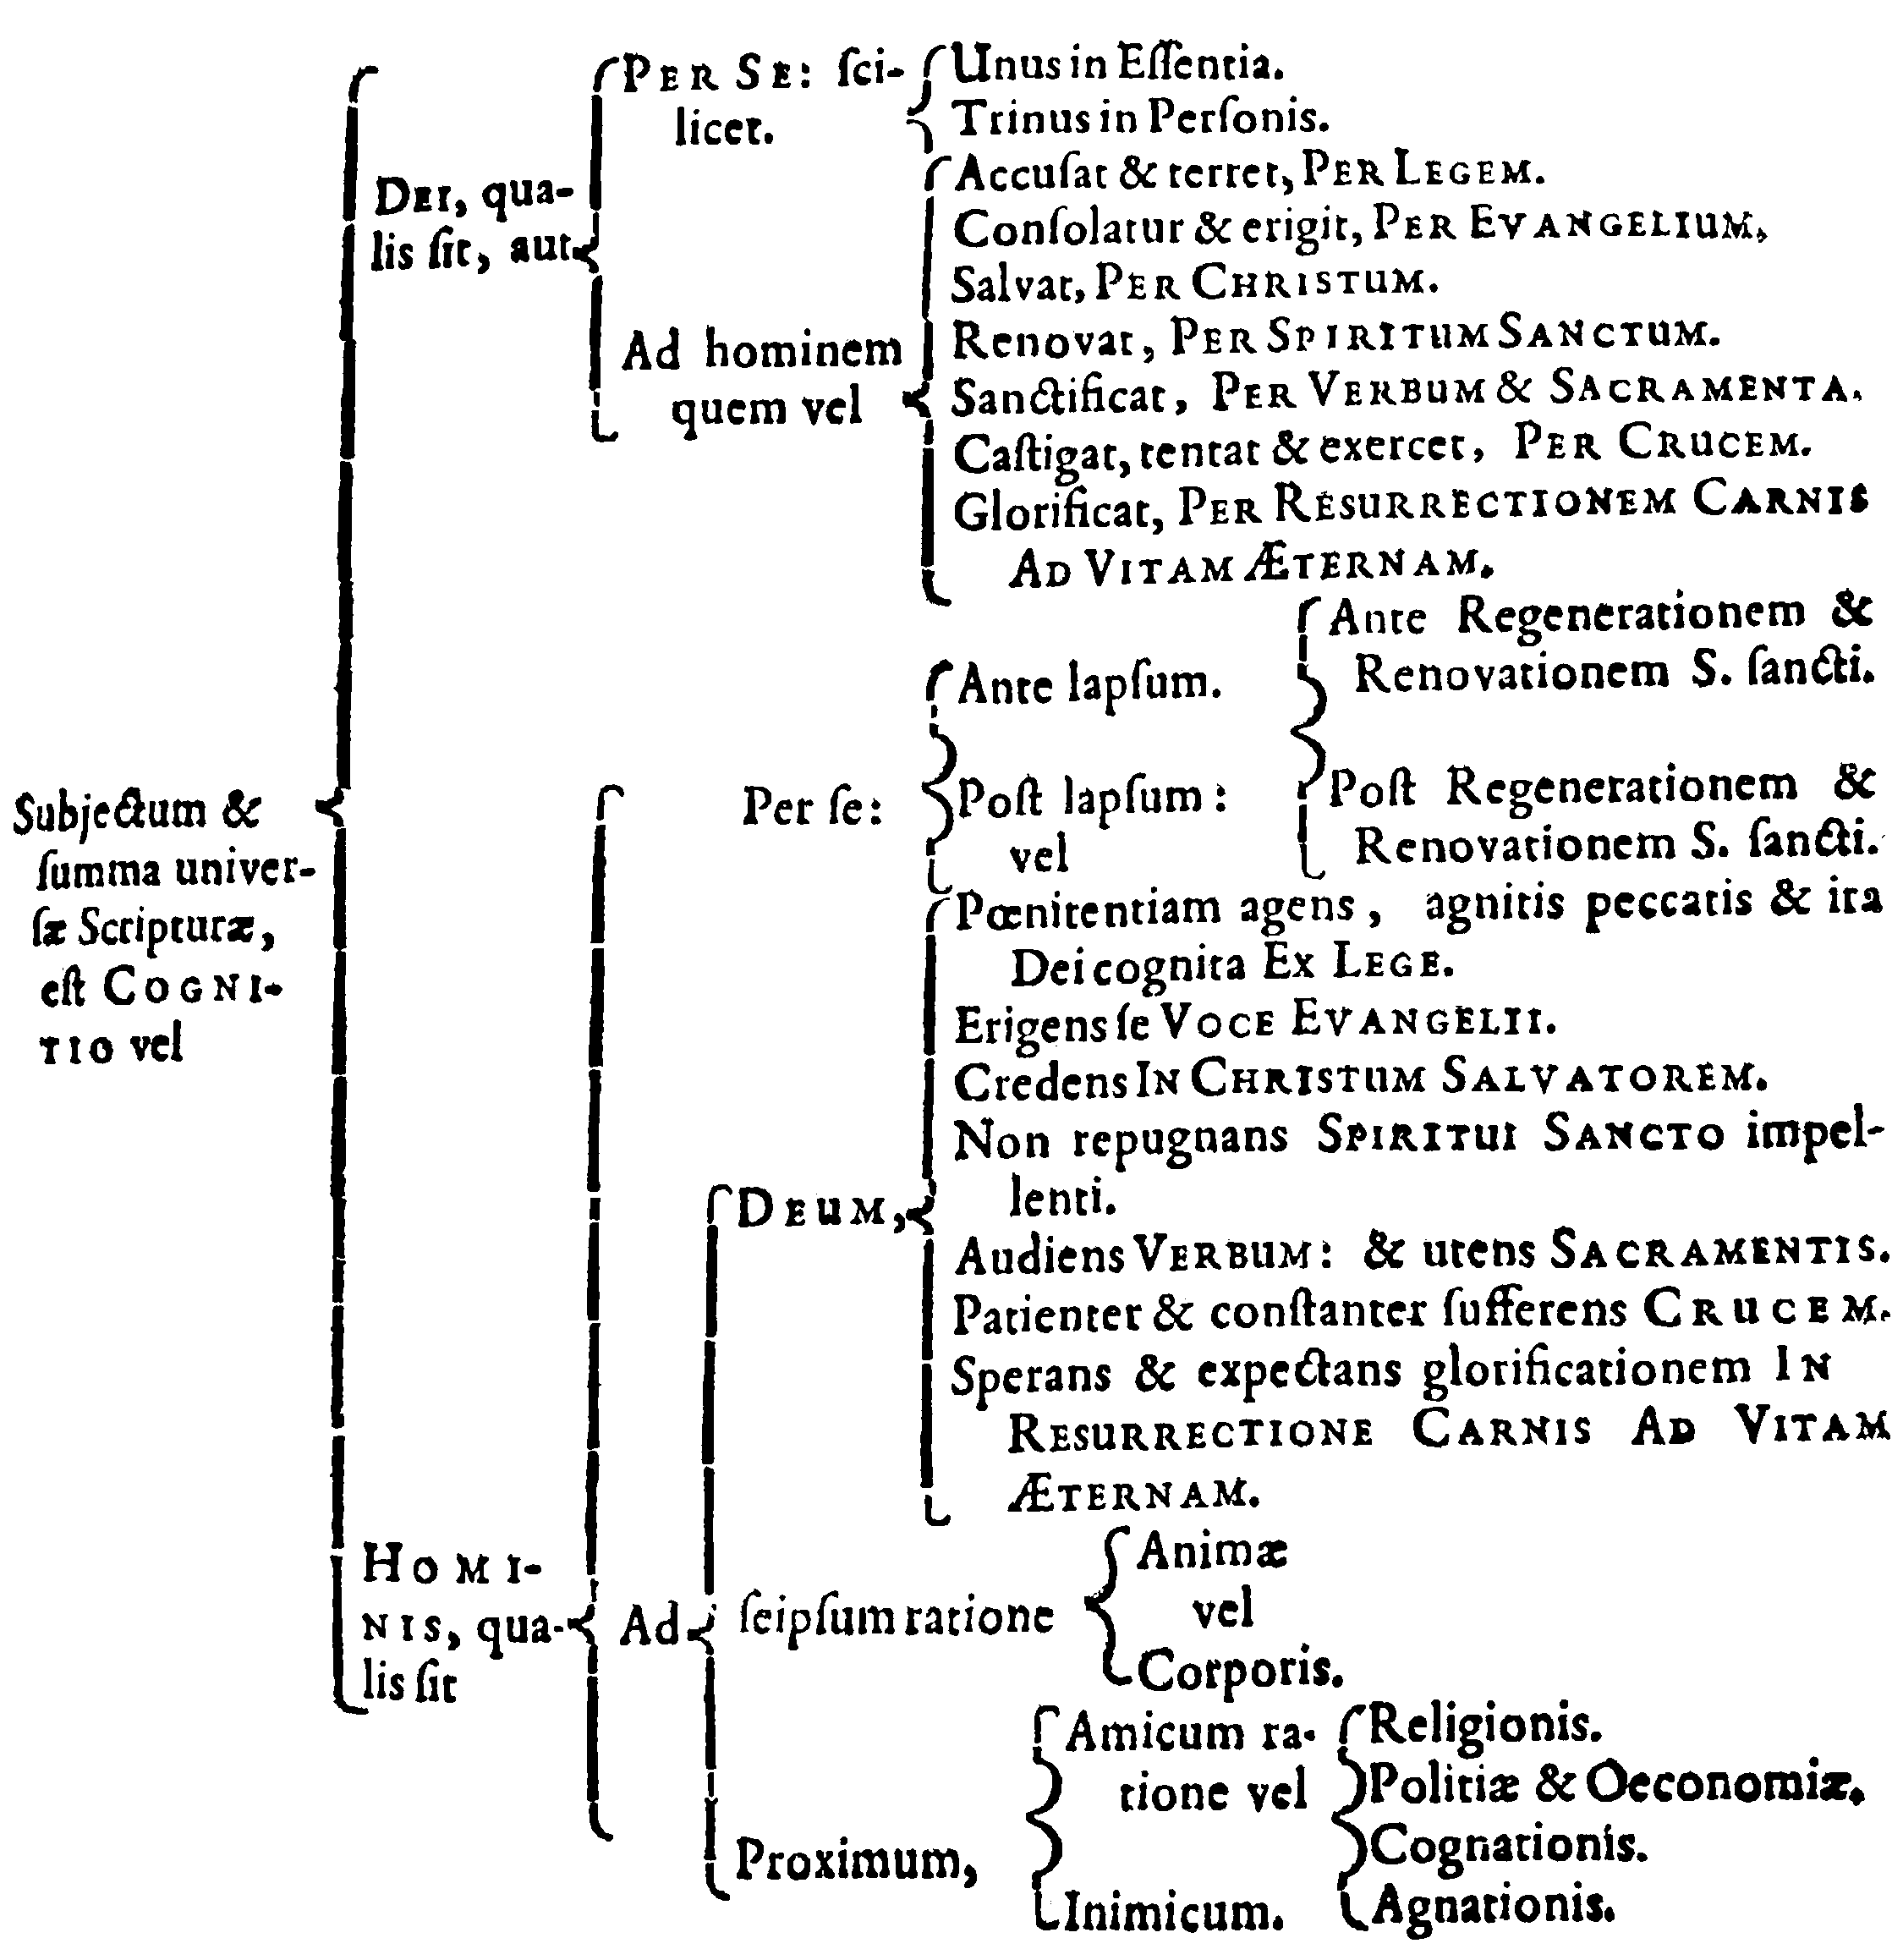
\includegraphics[width=\textwidth]{schemata.png}\bigskip
%
% \begin{itemize}
% \item As you see, the braces were composed of various type sorts, mainly smaller rules and assorted curly and bendy bits.
% 
% \item Because this is Latin we will see roman, italic and small caps, but little of other typefaces. We do see \emph{s-medialis} and many old-style ligatures.
% 
% \item In the reproduction we will use \emph{s-finalis} only, but we will retain some ligatures.
% 
% \item We will improve spacing between elements.
% 
% \item We will not aim for an exact reproduction of line breaks and such.
% \end{itemize}
% \newpage
% 
% We begin by looking at the ``leaves,'' the rightmost bits of text enclosed by braces. We can use \cmd{\schema} in these cases. That results in the following:
% 
% \begin{quote}
% \StartNum
% \begin{verbatim}
% \schema
% {\schemabox{\textsc{Per se}:\\ scilicet.}}
% {
%   \schemabox{Unus in essentia.}
%   \schemabox{Trinus in personis.}
% }\end{verbatim}
% \qquad\schema
% {\schemabox{\textsc{Per se}:\\ scilicet.}}
% {
%   \schemabox{Unus in essentia.}
%   \schemabox{Trinus in personis.}
% }
% \end{quote}
%
% \begin{quote}
% \StartNum
% \begin{verbatim}
%\schema
%{\schemabox{Ad hominem\\ quem vel}}
%{
%  \schemabox{Accusat \& terret, \textsc{Per Legem},\\
%  Consolatur \& erigit, \textsc{Per Evangelium}.\\
%  Salvat, \textsc{Per Christum}.\\
%  Renovat, \textsc{Per Spiritum Sanctum}.\\
%  Sanctificat, \textsc{Per Verbum} \& \textsc{Sacramenta}.\\
%  Castigat, tentat \& exercet, \textsc{Per Crucem}.\\
%  Glorificat \textsc{Per Resurrectionem Carnis}\\
%  \textsc{\quad Ad Vitam \AE{}ternam}.}
%}\end{verbatim}
% \qquad\schema
% {\schemabox{Ad hominem\\ quem vel}}
% {
%   \schemabox{Accusat \& terret, \textsc{Per Legem},\\
%   Consolatur \& erigit, \textsc{Per Evangelium}.\\
%   Salvat, \textsc{Per Christum}.\\
%   Renovat, \textsc{Per Spiritum Sanctum}.\\
%   Sanctificat, \textsc{Per Verbum} \& \textsc{Sacramenta}.\\
%   Castigat, tentat \& exercet, \textsc{Per Crucem}.\\
%   Glorificat \textsc{Per Resurrectionem Carnis}\\
%   \textsc{\quad Ad Vitam \AE{}ternam}.}
% }
% \end{quote}
%
% \begin{quote}
% \StartNum
% \begin{verbatim}
%\schemabox{Ante lapsum.}
%       
%\schema
%{\schemabox{Post lapsum:}}
%{
%  \schemabox{Ante Regenerationem \&\\
%  Renovationem S. Sancti.}
%  \schemabox{Post Regenerationem \&\\
%  Renovationem S. Sancti.}
%}\end{verbatim}
% \qquad\schemabox{Ante lapsum.}\footnote{We delete line 2 after \emph{Ante lapsum} in the large example on page~\pageref{page:firstbig} and thereafter.}
% 
% \qquad\schema
% {\schemabox{Post lapsum:}}
% {
%   \schemabox{Ante Regenerationem \&\\
%   Renovationem S. Sancti.}
%   \schemabox{Post Regenerationem \&\\
%   Renovationem S. Sancti.}
% }
% \end{quote}
% \newpage
%
% \begin{quote}
% \StartNum
% \begin{verbatim}
%\schema
%{\schemabox{\textsc{Deum},}}
%{
%  \schemabox{P\oe{}nitentia agens, agnitis peccatis \&\\
%  ira Dei cognita \textsc{Ex Lege}.\\
%  Erigens se \textsc{Voce Evangelii}.\\
%  Credens \textsc{In Christum Salvatorem}.\\
%  Non repugnans \textsc{Spiritui Sancto} impellenti.\\
%  Audiens \textsc{Verbum}: \& utens \textsc{Sacramentis}.\\
%  Patienter \& constanter sufferens \textsc{Crucem}.\\
%  Sperans \& expectans glorificationem\\
%  \textsc{\quad In Resurrectione Carnis}\\
%  \textsc{\quad Ad Vitam \AE{}ternam}.}
%}\end{verbatim}
% \qquad\schema
% {\schemabox{\textsc{Deum},}}
% {
%   \schemabox{P\oe{}nitentia agens, agnitis peccatis \&\\
%   ira Dei cognita \textsc{Ex Lege}.\\
%   Erigens se \textsc{Voce Evangelii}.\\
%   Credens \textsc{In Christum Salvatorem}.\\
%   Non repugnans \textsc{Spiritui Sancto} impellenti.\\
%   Audiens \textsc{Verbum}: \& utens \textsc{Sacramentis}.\\
%   Patienter \& constanter sufferens \textsc{Crucem}.\\
%   Sperans \& expectans glorificationem\\
%   \textsc{\quad In Resurrectione Carnis}\\
%   \textsc{\quad Ad Vitam \AE{}ternam}.}
% }
% \end{quote}
%
% \begin{quote}
% \StartNum
% \begin{verbatim}
%\schema
%{\schemabox{seipsum ratione}}
%{\schemabox{Anim\ae{}\\ vel\\ Corporis}}\end{verbatim}
% \qquad\schema
% {\schemabox{seipsum ratione}}
% {\schemabox{Anim\ae{}\\ vel\\ Corporis}}
% \end{quote}
%
% \begin{quote}
% \StartNum
% \begin{verbatim}
%\schema
%{\schemabox{Amicum ra-\\ tione vel}}
%{
%  \schemabox{Religionis.\\
%  Politic\ae{} \& \OE{}conomic\ae{}.\\
%  Cognationis.\\
%  Agnationis.}
%}
%
%\schemabox{Inimicum.}\end{verbatim}
% \qquad\schema
% {\schemabox{Amicum ra-\\ tione vel}}
% {
%   \schemabox{Religionis.\\
%   Politic\ae{} \& \OE{}conomic\ae{}.\\
%   Cognationis.\\
%   Agnationis.}
% }
% 
% \qquad\schemabox{Inimicum.}\footnote{We delete line 9 before \emph{Inimicum} in the large example on page~\pageref{page:firstbig} and thereafter.}
% \end{quote}
% \newpage
% 
% \phantomsection
% \label{page:firstbig}
% Below we build all of the ``leaves'' into the larger schema using \cmd{\Schema}. The braces all have dummy values of \texttt{0ex} \meta{adjust} and \texttt{5ex} \meta{size}. Please do not be alarmed at how bad this looks right now! We will adjust the layout shortly. We just want to see the general look of things:\bigskip
%
% \bgroup\small\begin{displaymath}
% \Schema{0ex}{5ex}
% {
%   \schemabox{Subjectum \&\\
%   summa univer-\\
%   s\ae{} Scriptur\ae{},\\
%   est \textsc{Cognitio}\\
%   vel}
% }
% {
%   \Schema{0ex}{5ex}
%   {
%     \schemabox{\textsc{Dei}, qua-\\lis sit, aut}
%   }
%   {
%     \schema
%     {\schemabox{\textsc{Per se}:\\ scilicet.}}
%     {
%       \schemabox{Unus in essentia.}
%       \schemabox{Trinus in personis.}
%     }
%     \schema
%     {\schemabox{Ad hominem\\ quem vel}}
%     {
%       \schemabox{Accusat \& terret, \textsc{Per Legem},\\
%       Consolatur \& erigit, \textsc{Per Evangelium}.\\
%       Salvat, \textsc{Per Christum}.\\
%       Renovat, \textsc{Per Spiritum Sanctum}.\\
%       Sanctificat, \textsc{Per Verbum} \& \textsc{Sacramenta}.\\
%       Castigat, tentat \& exercet, \textsc{Per Crucem}.\\
%       Glorificat \textsc{Per Resurrectionem Carnis}\\
%       \textsc{\quad Ad Vitam \AE{}ternam}.}
%     }
%   }
%   \Schema{0ex}{5ex}
%   {
%     \schemabox{\textsc{Hominis},\\ qualis sit}
%   }
%   {
%     \Schema{0ex}{5ex}
%     {\schemabox{\textsc{Per se}:}}
%     {
%       \schemabox{Ante lapsum.}
%       \schema
%       {\schemabox{Post lapsum:}}
%       {
%         \schemabox{Ante Regenerationem \&\\
%         Renovationem S. Sancti.}
%         \schemabox{Post Regenerationem \&\\
%         Renovationem S. Sancti.}
%       }
%     }
%     \Schema{0ex}{5ex}
%     {\schemabox{Ad}}
%     {
%       \schema
%       {\schemabox{\textsc{Deum},}}
%       {
%         \schemabox{P\oe{}nitentia agens, agnitis peccatis \&\\
%         ira Dei cognita \textsc{Ex Lege}.\\
%         Erigens se \textsc{Voce Evangelii}.\\
%         Credens \textsc{In Christum Salvatorem}.\\
%         Non repugnans \textsc{Spiritui Sancto} impellenti.\\
%         Audiens \textsc{Verbum}: \& utens \textsc{Sacramentis}.\\
%         Patienter \& constanter sufferens \textsc{Crucem}.\\
%         Sperans \& expectans glorificationem\\
%         \textsc{\quad In Resurrectione Carnis}\\
%         \textsc{\quad Ad Vitam \AE{}ternam}.}
%       }
%       \schema
%         {\schemabox{seipsum ratione}}
%         {\schemabox{Anim\ae{}\\ vel\\ Corporis}}
%       \Schema{0ex}{5ex}
%       {\schemabox{Proximum,}}
%       {
%         \schema
%         {\schemabox{Amicum ra-\\ tione vel}}
%         {
%           \schemabox{Religionis.\\
%           Politic\ae{} \& \OE{}conomic\ae{}.\\
%           Cognationis.\\
%           Agnationis.}
%         }
%         \schemabox{Inimicum.}
%       }
%     }
%   }
% }
%\end{displaymath}\egroup\bigskip
%
% Below we have the code listing for the schema above. One can see that there is much correlation between the listing and the printed result:
%
% \begin{quote}\small
% \StartNum
% \begin{verbatim}
%\Schema{0ex}{5ex}
%{
%  \schemabox{Subjectum \&\\
%  summa univer-\\
%  s\ae{} Scriptur\ae{},\\
%  est \textsc{Cognitio}\\
%  vel}
%}
%{
%  \Schema{0ex}{5ex}
%  {
%    \schemabox{\textsc{Dei}, qua-\\lis sit, aut}
%  }
%  {
%    \schema
%    {\schemabox{\textsc{Per se}:\\ scilicet.}}
%    {
%      \schemabox{Unus in essentia.}
%      \schemabox{Trinus in personis.}
%    }
%    \schema
%    {\schemabox{Ad hominem\\ quem vel}}
%    {
%      \schemabox{Accusat \& terret, \textsc{Per Legem},\\
%      Consolatur \& erigit, \textsc{Per Evangelium}.\\
%      Salvat, \textsc{Per Christum}.\\
%      Renovat, \textsc{Per Spiritum Sanctum}.\\
%      Sanctificat, \textsc{Per Verbum} \& \textsc{Sacramenta}.\\
%      Castigat, tentat \& exercet, \textsc{Per Crucem}.\\
%      Glorificat \textsc{Per Resurrectionem Carnis}\\
%      \textsc{\quad Ad Vitam \AE{}ternam}.}
%    }
%  }
%  \Schema{0ex}{5ex}
%  {
%    \schemabox{\textsc{Hominis},\\ qualis sit}
%  }
%  {
%    \Schema{0ex}{5ex}
%    {\schemabox{\textsc{Per se}:}}
%    {
%      \schemabox{Ante lapsum.}
%      \schema
%      {\schemabox{Post lapsum:}}
%      {
%        \schemabox{Ante Regenerationem \&\\
%        Renovationem S. Sancti.}
%        \schemabox{Post Regenerationem \&\\
%        Renovationem S. Sancti.}
%      }
%    }
%    \Schema{0ex}{5ex}
%    {\schemabox{Ad}}
%    {
%      \schema
%      {\schemabox{\textsc{Deum},}}
%      {
%        \schemabox{P\oe{}nitentia agens, agnitis peccatis \&\\
%        ira Dei cognita \textsc{Ex Lege}.\\
%        Erigens se \textsc{Voce Evangelii}.\\
%        Credens \textsc{In Christum Salvatorem}.\\
%        Non repugnans \textsc{Spiritui Sancto} impellenti.\\
%        Audiens \textsc{Verbum}: \& utens \textsc{Sacramentis}.\\
%        Patienter \& constanter sufferens \textsc{Crucem}.\\
%        Sperans \& expectans glorificationem\\
%        \textsc{\quad In Resurrectione Carnis}\\
%        \textsc{\quad Ad Vitam \AE{}ternam}.}
%      }
%      \schema
%        {\schemabox{seipsum ratione}}
%        {\schemabox{Anim\ae{}\\ vel\\ Corporis}}
%      \Schema{0ex}{5ex}
%      {\schemabox{Proximum,}}
%      {
%        \schema
%        {\schemabox{Amicum ra-\\ tione vel}}
%        {
%          \schemabox{Religionis.\\
%          Politic\ae{} \& \OE{}conomic\ae{}.\\
%          Cognationis.\\
%          Agnationis.}
%        }
%        \schemabox{Inimicum.}
%      }
%    }
%  }
%}\end{verbatim}
% \end{quote}
%
% First, we add space between the ``leaves'' of the tree. If you do not work from right to left, you will waste time revising the ``leaves'' and ``branches.'' The following lines, shown with some surrounding context, were changed.
%
% Remember that you can add a \cmd{\smallskip} within a \cmd{\schemabox} in \LaTeX{}, but not in \PlainTeX. We have split the text below into two boxes to make it format-agnostic. See also how the second \cmd{\smallskip} follows the closing brace of the right-hand side, not the \cmd{\schemabox.} That adjusts the entire \cmd{\schema}.
% \begin{quote}\small\StartNum\addtocounter{VerbLine}{16}
% \begin{verbatim}
%    {
%      \schemabox{Unus in essentia.}\smallskip
%      \schemabox{Trinus in personis.}
%    }\smallskip\end{verbatim}
% \end{quote}
% 
% Again, below, the skip comes at the close of a \cmd{\schema}.
% \begin{quote}\small\ContinueNum\addtocounter{VerbLine}{10}
% \begin{verbatim}
%      \textsc{\quad Ad Vitam \AE{}ternam}.}
%    }\medskip\end{verbatim}
% \end{quote}
% 
% Below, the first skip helps to separate the lone \cmd{\schemabox} from the \cmd{\schema} beneath it. This illustrates how the internal vertical lists of schemata can contain heterogeneous material.
% 
% A medium skip is placed between two \cmd{\schemabox}es, which slightly throws off the way the brace spans the boxes. A small skip is put at the end of the last \cmd{\schemabox} to correct that. Sometimes putting skips within a \cmd{\schema} can be tricky. Then a \cmd{\smallskip} is added again at the end of the right-hand side.
% \begin{quote}\small\ContinueNum\addtocounter{VerbLine}{8}
% \begin{verbatim}
%    {
%      \schemabox{Ante lapsum.}\smallskip
%      \schema
%      {\schemabox{Post lapsum:}}
%      {
%        \schemabox{Ante Regenerationem \&\\
%        Renovationem S. Sancti.}\medskip
%        \schemabox{Post Regenerationem \&\\
%        Renovationem S. Sancti.}\smallskip
%      }\smallskip
%    }\end{verbatim}
% \end{quote}
% 
% The skips below generally follow the same patterns that we have seen above.
% \begin{quote}\small\ContinueNum\addtocounter{VerbLine}{15}
% \begin{verbatim}
%        \textsc{\quad Ad Vitam \AE{}ternam}.}
%      }\smallskip
%      \schema
%        {\schemabox{seipsum ratione}}
%        {\schemabox{Anim\ae{}\\ vel\\ Corporis}}\smallskip\end{verbatim}
% \end{quote}
% 
% \begin{quote}\small\ContinueNum\addtocounter{VerbLine}{10}
% \begin{verbatim}
%          }\smallskip
%          \schemabox{Inimicum.}\end{verbatim}
% \end{quote}
%
%The resulting schema looks better already:
% \bgroup\small\begin{displaymath}
% \Schema{0ex}{5ex}
% {
%   \schemabox{Subjectum \&\\
%   summa univer-\\
%   s\ae{} Scriptur\ae{},\\
%   est \textsc{Cognitio}\\
%   vel}
% }
% {
%   \Schema{0ex}{5ex}
%   {
%     \schemabox{\textsc{Dei}, qua-\\lis sit, aut}
%   }
%   {
%     \schema
%     {\schemabox{\textsc{Per se}:\\ scilicet.}}
%     {
%       \schemabox{Unus in essentia.}\smallskip
%       \schemabox{Trinus in personis.}
%     }\smallskip
%     \schema
%     {\schemabox{Ad hominem\\ quem vel}}
%     {
%       \schemabox{Accusat \& terret, \textsc{Per Legem},\\
%       Consolatur \& erigit, \textsc{Per Evangelium}.\\
%       Salvat, \textsc{Per Christum}.\\
%       Renovat, \textsc{Per Spiritum Sanctum}.\\
%       Sanctificat, \textsc{Per Verbum} \& \textsc{Sacramenta}.\\
%       Castigat, tentat \& exercet, \textsc{Per Crucem}.\\
%       Glorificat \textsc{Per Resurrectionem Carnis}\\
%       \textsc{\quad Ad Vitam \AE{}ternam}.}
%     }\medskip
%   }
%   \Schema{0ex}{5ex}
%   {
%     \schemabox{\textsc{Hominis},\\ qualis sit}
%   }
%   {
%     \Schema{0ex}{5ex}
%     {\schemabox{\textsc{Per se}:}}
%     {
%       \schemabox{Ante lapsum.}\smallskip
%       \schema
%       {\schemabox{Post lapsum:}}
%       {
%         \schemabox{Ante Regenerationem \&\\
%         Renovationem S. Sancti.}\medskip
%         \schemabox{Post Regenerationem \&\\
%         Renovationem S. Sancti.}\smallskip
%       }\smallskip
%     }
%     \Schema{0ex}{5ex}
%     {\schemabox{Ad}}
%     {
%       \schema
%       {\schemabox{\textsc{Deum},}}
%       {
%         \schemabox{P\oe{}nitentia agens, agnitis peccatis \&\\
%         ira Dei cognita \textsc{Ex Lege}.\\
%         Erigens se \textsc{Voce Evangelii}.\\
%         Credens \textsc{In Christum Salvatorem}.\\
%         Non repugnans \textsc{Spiritui Sancto} impellenti.\\
%         Audiens \textsc{Verbum}: \& utens \textsc{Sacramentis}.\\
%         Patienter \& constanter sufferens \textsc{Crucem}.\\
%         Sperans \& expectans glorificationem\\
%         \textsc{\quad In Resurrectione Carnis}\\
%         \textsc{\quad Ad Vitam \AE{}ternam}.}
%       }\smallskip
%       \schema
%         {\schemabox{seipsum ratione}}
%         {\schemabox{Anim\ae{}\\ vel\\ Corporis}}\smallskip
%       \Schema{0ex}{5ex}
%       {\schemabox{Proximum,}}
%       {
%         \schema
%         {\schemabox{Amicum ra-\\ tione vel}}
%         {
%           \schemabox{Religionis.\\
%           Politic\ae{} \& \OE{}conomic\ae{}.\\
%           Cognationis.\\
%           Agnationis.}
%         }\smallskip
%         \schemabox{Inimicum.}
%       }
%     }
%   }
% }
%\end{displaymath}\egroup
% \newpage
% 
% \newpage
% 
% Next we estimate the lines of text and blank lines from the top of a \cmd{\Schema} brace to the bottom, e.g., from ``\textsc{Per se}:'' to ``quem vel''. We use those ``ex'' height figures for \meta{size}. The following lines illustrate our ``ball park'' figures:
%
% \begin{quote}\small\StartNum
% \begin{verbatim}
% \Schema{0ex}{23ex}\end{verbatim}
% \end{quote}
% \begin{quote}\small\ContinueNum\addtocounter{VerbLine}{8}
% \begin{verbatim}
% \Schema{0ex}{8ex}\end{verbatim}
% \end{quote}
% \begin{quote}\small\ContinueNum\addtocounter{VerbLine}{23}
% \begin{verbatim}
% \Schema{0ex}{16ex}\end{verbatim}
% \end{quote}
% \begin{quote}\small\ContinueNum\addtocounter{VerbLine}{4}
% \begin{verbatim}
% \Schema{0ex}{5ex}\end{verbatim}
% \end{quote}
% \begin{quote}\small\ContinueNum\addtocounter{VerbLine}{12}
% \begin{verbatim}
% \Schema{0ex}{16ex}\end{verbatim}
% \end{quote}
% \begin{quote}\small\ContinueNum\addtocounter{VerbLine}{19}
% \begin{verbatim}
% \Schema{0ex}{5ex}\end{verbatim}
% \end{quote}
% 
% \bgroup\small\begin{displaymath}
% \Schema{0ex}{23ex}
% {
%   \schemabox{Subjectum \&\\
%   summa univer-\\
%   s\ae{} Scriptur\ae{},\\
%   est \textsc{Cognitio}\\
%   vel}
% }
% {
%   \Schema{-6.4ex}{8.6ex}
%   {
%     \schemabox{\textsc{Dei}, qua-\\lis sit, aut}
%   }
%   {
%     \schema
%     {\schemabox{\textsc{Per se}:\\ scilicet.}}
%     {
%       \schemabox{Unus in essentia.}\smallskip
%       \schemabox{Trinus in personis.}
%     }\smallskip
%     \schema
%     {\schemabox{Ad hominem\\ quem vel}}
%     {
%       \schemabox{Accusat \& terret, \textsc{Per Legem},\\
%       Consolatur \& erigit, \textsc{Per Evangelium}.\\
%       Salvat, \textsc{Per Christum}.\\
%       Renovat, \textsc{Per Spiritum Sanctum}.\\
%       Sanctificat, \textsc{Per Verbum} \& \textsc{Sacramenta}.\\
%       Castigat, tentat \& exercet, \textsc{Per Crucem}.\\
%       Glorificat \textsc{Per Resurrectionem Carnis}\\
%       \textsc{\quad Ad Vitam \AE{}ternam}.}
%     }\medskip
%   }
%   \Schema{0ex}{16ex}
%   {
%     \schemabox{\textsc{Hominis},\\ qualis sit}
%   }
%   {
%     \Schema{0ex}{5ex}
%     {\schemabox{\textsc{Per se}:}}
%     {
%       \schemabox{Ante lapsum.}\smallskip
%       \schema
%       {\schemabox{Post lapsum:}}
%       {
%         \schemabox{Ante Regenerationem \&\\
%         Renovationem S. Sancti.}\medskip
%         \schemabox{Post Regenerationem \&\\
%         Renovationem S. Sancti.}\smallskip
%       }\smallskip
%     }
%     \Schema{0ex}{16ex}
%     {\schemabox{Ad}}
%     {
%       \schema
%       {\schemabox{\textsc{Deum},}}
%       {
%         \schemabox{P\oe{}nitentia agens, agnitis peccatis \&\\
%         ira Dei cognita \textsc{Ex Lege}.\\
%         Erigens se \textsc{Voce Evangelii}.\\
%         Credens \textsc{In Christum Salvatorem}.\\
%         Non repugnans \textsc{Spiritui Sancto} impellenti.\\
%         Audiens \textsc{Verbum}: \& utens \textsc{Sacramentis}.\\
%         Patienter \& constanter sufferens \textsc{Crucem}.\\
%         Sperans \& expectans glorificationem\\
%         \textsc{\quad In Resurrectione Carnis}\\
%         \textsc{\quad Ad Vitam \AE{}ternam}.}
%       }\smallskip
%       \schema
%         {\schemabox{seipsum ratione}}
%         {\schemabox{Anim\ae{}\\ vel\\ Corporis}}\smallskip
%       \Schema{0ex}{5ex}
%       {\schemabox{Proximum,}}
%       {
%         \schema
%         {\schemabox{Amicum ra-\\ tione vel}}
%         {
%           \schemabox{Religionis.\\
%           Politic\ae{} \& \OE{}conomic\ae{}.\\
%           Cognationis.\\
%           Agnationis.}
%         }\smallskip
%         \schemabox{Inimicum.}
%       }
%     }
%   }
% }
%\end{displaymath}\egroup
%
% \newpage
% 
% Next we tweak \meta{adjust} values by counting the lines (\texttt{ex}) in the direction the left side needs to move relative to the right, multiply the result by two, and make it negative for up and positive for down. Using an editor, e.g., \texttt{texworks} makes this fairly easy. We also adjust the final \meta{size} of the braces. Work from leaves to root:
% \begin{quote}\small\StartNum
% \begin{verbatim}
% \Schema{-25ex}{20.6ex}% Do this one last. ``Subjectum''\end{verbatim}
% \end{quote}
% \begin{quote}\small\ContinueNum\addtocounter{VerbLine}{8}
% \begin{verbatim}
% \Schema{-6.4ex}{8.5ex}% Do this one first. ``Dei''\end{verbatim}
% \end{quote}
% \begin{quote}\small\ContinueNum\addtocounter{VerbLine}{23}
% \begin{verbatim}
% \Schema{-13.4ex}{17.4ex}% Do this one fifth. ``Hominis''\end{verbatim}
% \end{quote}
% \begin{quote}\small\ContinueNum\addtocounter{VerbLine}{4}
% \begin{verbatim}
% \Schema{-4.4ex}{5ex}% Do this one second. ``Per se'' (lower)\end{verbatim}
% \end{quote}
% \begin{quote}\small\ContinueNum\addtocounter{VerbLine}{12}
% \begin{verbatim}
% \Schema{4.2ex}{14.4ex}% Do this one fourth. ``Ad''\end{verbatim}
% \end{quote}
% \begin{quote}\small\ContinueNum\addtocounter{VerbLine}{19}
% \begin{verbatim}
% \Schema{2ex}{5.1ex}% Do this one third. ``Proximum''\end{verbatim}
% \end{quote}
%
% \bgroup\small\begin{displaymath}
% \Schema{-25ex}{20.6ex}
% {
%   \schemabox{Subjectum \&\\
%   summa univer-\\
%   s\ae{} Scriptur\ae{},\\
%   est \textsc{Cognitio}\\
%   vel}
% }
% {
%   \Schema{-6.4ex}{8.5ex}
%   {
%     \schemabox{\textsc{Dei}, qua-\\lis sit, aut}
%   }
%   {
%     \schema
%     {\schemabox{\textsc{Per se}:\\ scilicet.}}
%     {
%       \schemabox{Unus in essentia.}\smallskip
%       \schemabox{Trinus in personis.}
%     }\smallskip
%     \schema
%     {\schemabox{Ad hominem\\ quem vel}}
%     {
%       \schemabox{Accusat \& terret, \textsc{Per Legem},\\
%       Consolatur \& erigit, \textsc{Per Evangelium}.\\
%       Salvat, \textsc{Per Christum}.\\
%       Renovat, \textsc{Per Spiritum Sanctum}.\\
%       Sanctificat, \textsc{Per Verbum} \& \textsc{Sacramenta}.\\
%       Castigat, tentat \& exercet, \textsc{Per Crucem}.\\
%       Glorificat \textsc{Per Resurrectionem Carnis}\\
%       \textsc{\quad Ad Vitam \AE{}ternam}.}
%     }\medskip
%   }
%   \Schema{-13.4ex}{17.4ex}
%   {
%     \schemabox{\textsc{Hominis},\\ qualis sit}
%   }
%   {
%     \Schema{-4.4ex}{5ex}
%     {\schemabox{\textsc{Per se}:}}
%     {
%       \schemabox{Ante lapsum.}\smallskip
%       \schema
%       {\schemabox{Post lapsum:}}
%       {
%         \schemabox{Ante Regenerationem \&\\
%         Renovationem S. Sancti.}\medskip
%         \schemabox{Post Regenerationem \&\\
%         Renovationem S. Sancti.}\smallskip
%       }\smallskip
%     }
%     \Schema{4.2ex}{14.4ex}
%     {\schemabox{Ad}}
%     {
%       \schema
%       {\schemabox{\textsc{Deum},}}
%       {
%         \schemabox{P\oe{}nitentia agens, agnitis peccatis \&\\
%         ira Dei cognita \textsc{Ex Lege}.\\
%         Erigens se \textsc{Voce Evangelii}.\\
%         Credens \textsc{In Christum Salvatorem}.\\
%         Non repugnans \textsc{Spiritui Sancto} impellenti.\\
%         Audiens \textsc{Verbum}: \& utens \textsc{Sacramentis}.\\
%         Patienter \& constanter sufferens \textsc{Crucem}.\\
%         Sperans \& expectans glorificationem\\
%         \textsc{\quad In Resurrectione Carnis}\\
%         \textsc{\quad Ad Vitam \AE{}ternam}.}
%       }\smallskip
%       \schema
%         {\schemabox{seipsum ratione}}
%         {\schemabox{Anim\ae{}\\ vel\\ Corporis}}\smallskip
%       \Schema{2ex}{5.1ex}
%       {\schemabox{Proximum,}}
%       {
%         \schema
%         {\schemabox{Amicum ra-\\ tione vel}}
%         {
%           \schemabox{Religionis.\\
%           Politic\ae{} \& \OE{}conomic\ae{}.\\
%           Cognationis.\\
%           Agnationis.}
%         }\smallskip
%         \schemabox{Inimicum.}
%       }
%     }
%   }
% }
%\end{displaymath}\egroup
%
% \subsubsection[Big Groups]{Big Schema with Groups}
%
% The next example illustrates everything tha we have covered so far, plus \cmd{\DoGroups}, all inside a local scope:\bigskip
% 
% \bgroup\footnotesize\begin{displaymath}
% \DoGroups%
%\Schema{-27ex}{21.5ex}
%{
%  \schemabox{Sacr\ae{}\\ litter\ae{}\\ loquuntur,\\ de}
%}
%{
%  \schema
%  {
%    \schemabox{\textsc{Deo}}
%  }
%  {
%    \schemabox{Uno, in Trinitate.}\smallskip\schemabox{Trino, in unitate.}
%  }
%  \Schema{-17ex}{23.4ex}
%  {
%    \vskip30ex
%    \schemabox{\textsc{Dei}\\ \textsc{Operibus}}
%  }
%  {
%    \schema
%    {
%      \schemabox{\textsc{Intra},\\ qu\ae{} sunt\\ divisa, ut}
%    }
%    {
%      \schemabox{\textsc{Patris}, ab \ae{}terno gignere.\\ \textsc{Filii}, ab \ae{}terno genitum esse.\\ \textsc{Spiritus Sancti}, ab utroque\\ ab \ae{}terno procedete.\strut}
%    }
%    \medskip
%    \Schema{-2ex}{21ex}
%    {
%      \schemabox{\textsc{Extra},\\ qu\ae{} sunt\\ indivisa;\\ tervata\\ tamen\\ cujusque\\ person\ae{}\\ divinitatis\\ sua pro-\\prietate}
%    }
%    {
%      \Schema{-0.8ex}{6.4ex}
%      {
%        \schemabox{Creatione\\ natur\ae{}}
%      }
%      {
%        \schema
%        {
%          \schemabox{Brute ut}
%        }
%        {
%          \schemabox{C\oe{}li} \smallskip \schemabox{Elementorum} \smallskip \schemabox{Mundi}
%        }
%        \smallskip
%        \schema
%        {
%          \schemabox{\gk{logik~hs}, ut}
%        }
%        {
%          \schemabox{Angelorum.} \smallskip \schemabox{Hominum: Ad\ae{},\\ Ev\ae{} \& procreatorum\\ exipsis.\strut}
%        }
%      }
%      \schema
%      {
%        \schemabox{Sustenatione\\ natur\ae{} laps\ae{},}
%      }
%      {
%        \schemabox{Angelorum malorum,} \smallskip \schemabox{Hominum: Ad\ae{}, Ev\ae{}\\ \& procreatorum exipsis.}
%      }
%      \Schema{2.6ex}{8.8ex}
%      {
%        \schemabox{Beneficiis\\ erga Ecc-\\ lesiam: ea\\ versantur\\ aut circa}
%      }
%      {
%        \Schema{2.2ex}{7ex}
%        {
%          \schemabox{Res, ut}
%        }
%        {
%          \schema
%          {
%            \schemabox{Verbum}
%          }
%          {
%            \schemabox{Legis} \smallskip \schemabox{Evangelii} \smallskip \schemabox{Sacramentorum}
%          }
%          \smallskip
%          \schema
%          {
%            \schemabox{Signa vel Veteris\\ vel Novi Testa-\\ mentum ut sunt:}
%          }
%          {
%            \schemabox{Ceremoni\ae{}} \smallskip \schemabox{Miracula}
%          }
%        }
%        \smallskip
%        \Schema{0.6ex}{5.5ex}
%        {
%          \schemabox{Personas}
%        }
%        {
%          \schema
%          {
%            \schemabox{Ecclesi\ae{}}
%          }
%          {
%            \schemabox{Universalis} \smallskip \schemabox{Particularis}
%          }
%          \smallskip
%          \schemabox{Politi\ae{} ut Magistratuum}
%          \smallskip
%          \schemabox{\OE{}conomi\ae{} ut privatorum}
%        }
%      }\vskip2ex
%    }
%  }
%}
%\end{displaymath}\egroup
%
% \subsubsection[Open and Closed]{Open and Closed Schemata}
%
% Now we look at schemata that have both open and closed braces. One must use \cmd{\Schema} to get delimiters to be the same height. These schemata take the form:
% \begin{quote}\ttfamily
% \cmd{\Schema}\{\textrm{\meta{adjust}}\}\{\textrm{\meta{height}}\}\\
% \{\textrm{\meta{$left_1$}}\}\\
% \{\\
% \hbox{}\quad\cmd{\Schema}[close]\{\textrm{\meta{adjust}}\}\{\textrm{\meta{height}}\}\\
% \hbox{}\quad\{\textrm{\meta{$left_2$}}\}\\
% \hbox{}\quad\{\textrm{\meta{$right_2$}}\}\\
% \}
% \end{quote}
% \newbox\mybox
% \def\Box#1{%^^A
%   \setbox\mybox=\hbox{\vrule\vbox{\hrule%^^A
%     \vfil\hbox{\strut\space #1\space}%^^A
%     \vfil\hrule}\vrule}%^^A
%   \dimen0=\ht\mybox%^^A
%   \advance\dimen0 by2ex%^^A
%   \hbox{\vrule\vbox to \dimen0{\hrule%^^A
%     \vfil\hbox{{\Large\strut}\space #1\space}%^^A
%     \vfil\hrule}\vrule}}
%
% \newpage
% We use a modified version of our \cmd{\Box} macro from above to show how each part nests within the other. Below we do not use \cmd{\NudgeSB} from Section~\ref{sec:tweakschema} because we are not using \cmd{\schemabox}; instead we directly add the kern: |\hbox{\Box{\,$left_2$}\kern0.2em}| within the closed schema. The result is:\medskip
% 
% \begin{quote}
%   \quad\Schema{0ex}{2ex}
%     {\Box{\,$left_1$}}
%     {%^^A
%       \Box{%^^A
%         \Schema[close]{0ex}{2ex}
%         {\hbox{\Box{\,$left_2$}\kern0.2em}}
%         {\Box{\,$right_2$}}%^^A
%       }%^^A
%     }
% \end{quote}\medskip
% 
%  Here is another, more complex example:\medskip
%
% \begin{displaymath}
% \Schema{0ex}{6ex}
% {\Box{a}}
% {%^^A
%   \Box{%^^A
%     \Schema[close]{0ex}{6ex}
%     {%^^A
%       \Box{%^^A
%         \Schema{0ex}{3ex}
%         {\Box{b}}
%         {%^^A
%           \Box{%^^A
%             \Schema[close]{0ex}{3ex}
%             {\hbox{\Box{c}\kern0.2em}}
%             {\Box{d}}
%           }
%         }
%       }
%     }
%     {\Box{e}}
%   }
% }
% \end{displaymath}\medskip
%
% \begin{quote}\small\StartNum\begin{verbatim}
%\newbox\mybox
%\def\Box#1{%
%  \setbox\mybox=\hbox{\vrule\vbox{\hrule%
%    \vfil\hbox{\strut\space #1\space}%
%    \vfil\hrule}\vrule}%
%  \dimen0=\ht\mybox%
%  \advance\dimen0 by2ex%
%  \hbox{\vrule\vbox to \dimen0{\hrule%
%    \vfil\hbox{{\Large\strut}\space #1\space}%
%    \vfil\hrule}\vrule}}
%\Schema{0ex}{6ex}
%{\Box{a}}
%{%
%  \Box{%
%    \Schema[close]{0ex}{6ex}
%    {%
%      \Box{%
%        \Schema{0ex}{3ex}
%        {\Box{b}}
%        {%
%          \Box{%
%            \Schema[close]{0ex}{3ex}
%            {\hbox{\Box{c}\kern0.2em}}
%            {\Box{d}}
%          }
%        }
%      }
%    }
%    {\Box{e}}
%  }
%}\end{verbatim}
% \end{quote}
%\newpage
%
% This is more of a real-world example. As above, one must use \cmd{\Schema} to prevent the opening braces from being slightly larger than the closing braces.
% 
% \bgroup\small\begin{displaymath}
% \Schema{-1.4ex}{10ex}
% {
%   \schemabox{Qu\ae{} sit\\ \textsc{Dei}, vel}
% }
% {
%   \Schema{-1ex}{5ex}
%   {
%     \schemabox{\textsc{Essentia}, in}
%   }
%   {
%     \vskip1ex\schemabox{Unitate divina,}
%     \medskip
%     \Schema{0ex}{3.4ex}
%     {
%       \schemabox{Tribus perso-\\ nis divinitatis}
%     }
%     {
%       \Schema[close]{0ex}{3.4ex}
%       {
%         \NudgeSB\schemabox{Patre,\\ Filio,\\ Spiritui Sancto}
%       }
%       {
%         \schemabox{\gk{<omoous'iois}\\ \& co\ae{}ternis}
%       }
%     }
%   }
%   \medskip
%   \Schema{-0.2ex}{6.4ex}
%   {
%     \schemabox{\textsc{Voluntas},\\ revelatur in\\ actione, sive}
%   }
%   {
%     \Schema{0ex}{3.4ex}
%     {
%       \schemabox{Universali}
%     }
%     {
%       \Schema[close]{0ex}{3.4ex}
%       {
%         \schemabox{Creationis,\\Sustenationis,\\ Propagationis,}
%       }
%       {
%         \schemabox{rerum creatarum.}
%       }
%     }
%     \medskip
%     \schema
%     {
%       \schemabox{Speciali, in beneficiis\\ erga Ecclesiam, eam}
%     }
%     {
%       \schemabox{Colligendo.\\ Justificando.\\
%       Conservando.\\ Glorificando.}
%     }
%   }
% }
% \end{displaymath}\egroup\smallskip
% 
% This listing of the previous example illustrates how one handles closed schemata. The macro \cmd{\gk} uses \textsf{babel} to create Greek text.
%
% \begin{quote}\small\StartNum
% \begin{verbatim}
%\Schema{-1.4ex}{10ex}
%{\schemabox{Qu\ae{} sit\\ \textsc{Dei}, vel}}
%{
%  \Schema{-1ex}{5ex}
%  {\schemabox{\textsc{Essentia}, in}}
%  {
%    \vskip1ex\schemabox{Unitate divina,}
%    \medskip
%    \Schema{0ex}{3.4ex}
%    {\schemabox{Tribus perso-\\ nis divinitatis}}
%    {
%      \Schema[close]{0ex}{3.4ex}
%      {\NudgeSB\schemabox{Patre,\\ Filio,\\ Spiritui Sancto}}
%      {\schemabox{\gk{<omoous'iois}\\ \& co\ae{}ternis}}
%    }
%  }
%  \medskip
%  \Schema{-0.2ex}{6.4ex}
%  {\schemabox{\textsc{Voluntas},\\ revelatur in\\ actione, sive}}
%  {
%    \Schema{0ex}{3.4ex}
%    {\schemabox{Universali}}
%    {
%      \Schema[close]{0ex}{3.4ex}
%      {\schemabox{Creationis,\\ Sustenationis,\\ Propagationis,}}
%      {\schemabox{rerum creatarum.}}
%    }
%    \medskip
%    \schema
%    {\schemabox{Speciali, in beneficiis\\ erga Ecclesiam, eam}}
%    {\schemabox{Colligendo.\\ Justificando.\\
%     Conservando.\\ Glorificando.}}
%  }
%}\end{verbatim}
% \end{quote}
% \newpage
% 
% \subsection{Final features}
% \label{sec:multiple}
% This final example illustrates how one can set the width of a \cmd{\schemabox}, and for what sort of use that might be. Below we invoke \cmd{\DoBrackets} after the start of the group containing the right-hand side of the first \cmd{\Schema}.
% 
% \bgroup\small\begin{displaymath}
% \Schema{-0.2ex}{14.4ex}
% {\schemabox{\bfseries Curricula\\\bfseries Texts}}
% {
%   \DoBrackets%
%^^A% Doable in LaTeX, not in Plain TeX, because \outer.
%^^A% \newbox\mybox%
%   \setbox\mybox=\hbox{\bfseries III. Philosophical }%
%   \dimen0=\wd\mybox%
%   \schema
%     {\schemabox[\dimen0]{\bfseries I. General\\Studies}}
%     {\schemabox{1. Collected Works\\2. Encyclopedias}}
%   \smallskip
%   \schema
%     {\schemabox[\dimen0]{\bfseries II. Literary\\Disciplines}}
%     {\schemabox{1. Philology\\
%      2. Historical Introduction\\
%      3. Literary Theory\\
%      4. Application}}
%   \smallskip
%   \schema
%       {\schemabox[\dimen0]{\bfseries III. Philosophical\\Disciplines}}
%       {\schemabox{1. Source Texts\\
%        2. History of Philosophy\\
%        3. General Surveys\\
%        4. Specific Studies}}
%   \smallskip
%   \schema
%       {\schemabox[\dimen0]{\bfseries IV. Historical\\Disciplines}}
%       {\schemabox{1. General Surveys\\
%        2. Specialized Works}}
% }
%\end{displaymath}\egroup
% 
% \begin{quote}\small
% \StartNum
% \begin{verbatim}
%\Schema{-0.2ex}{14.4ex}
%{\schemabox{\bfseries Curricula\\\bfseries Texts}}
%{
%  \DoBrackets%
%  % \newbox here is doable in LaTeX, not in Plain TeX,
%  % where it must be used as an \outer macro.
%  \newbox\mybox%
%  \setbox\mybox=\hbox{\bfseries III. Philosophical }%
%  \dimen0=\wd\mybox%
%  \schema
%    {\schemabox[\dimen0]{\bfseries I. General\\Studies}}
%    {\schemabox{1. Collected Works\\2. Encyclopedias}}
%  \smallskip
%  \schema
%    {\schemabox[\dimen0]{\bfseries II. Literary\\Disciplines}}
%    {\schemabox{1. Philology\\
%     2. Historical Introduction\\
%     3. Literary Theory\\
%     4. Application}}
%  \smallskip
%  \schema
%    {\schemabox[\dimen0]{\bfseries III. Philosophical\\Disciplines}}
%    {\schemabox{1. Source Texts\\
%     2. History of Philosophy\\
%     3. General Surveys\\
%     4. Specific Studies}}
%  \smallskip
%  \schema
%    {\schemabox[\dimen0]{\bfseries IV. Historical\\Disciplines}}
%    {\schemabox{1. General Surveys\\
%     2. Specialized Works}}
%}\end{verbatim}
% \end{quote}
% \newpage
% 
%\StopEventually{^^A
%  \newgeometry{textwidth=160mm,textheight=237mm,right=25mm}
%  \newpage\PrintChanges
%  \newpage\PrintIndex
%}
% \iffalse
%<*package>
% \fi
% \section{Implementation}
%
% Shorter macros are written in both \LaTeX{} and generic \TeX. Longer macros implement a platform-specific front end and a common back end. The macros default to \LaTeXe{} format. If the format test fails, then generic macros are selected.\medskip
%
% \bgroup\footnotesize\obeylines
% \leavevmode\llap{\scriptsize 1\ \ }\verb+%<package>{\expandafter}\expandafter\ifx \csname schemataLaTeX\endcsname\relax+
% \leavevmode\llap{\scriptsize 2\ \ }\verb+%<package>  \def\schemataLaTeX{LaTeX2e}\fi+
% \leavevmode\llap{\scriptsize 3\ \ }\verb+%<package>\ifx\fmtname\schemataLaTeX+
% \leavevmode\llap{\scriptsize 4\ \ }\verb+%<package>\expandafter\NeedsTeXFormat\expandafter{\schemataLaTeX}+
% \leavevmode\llap{\scriptsize 5\ \ }\verb+%<package>\ProvidesPackage{schemata}+
%                                  \verb+%<*package>+
% \leavevmode\llap{\scriptsize 6\ \ }\verb+  [2020/03/14 v1.1 generic package to aid construction of topical categories]+
%                                  \verb+%</package>+
% \leavevmode\llap{\scriptsize 7\ \ }\verb+%<package>\fi+
% \egroup
% \makeatletter\advance\c@CodelineNo by 7\makeatother
% 
% \subsection{Internal Variables}
%
% \changes{v1.0}{2020/03/13}{current format handling}
% If we are not using \LaTeXe, we do the equivalent of \cmd{\makeatletter}.
% 
%    \begin{macrocode}
\ifx\fmtname\schemataLaTeX\else
  \catcode`@=11\relax
\fi
%    \end{macrocode}
%    
% \changes{v0.8}{2016/01/25}{Rename box/dimen registers}
% \changes{v1.0}{2020/03/13}{Rename box/dimen registers}
%Two box registers and two dimen registers are used to analyze the left-hand and right-hand vertical sizes of the boxes in a schema. To make it less likely for these internal variables to be redefined, they are now more ``unique.''
%
%    \begin{macrocode}
\newbox\@schemata@rhs
\newbox\@schemata@lhs
\newdimen\@schemata@rheight
\newdimen\@schemata@lheight
%    \end{macrocode}
%
% \changes{v0.6}{2013/03/10}{Added UC/LC tweaks.}
% \changes{v0.8}{2016/01/25}{Renamed internal macros}
% Two Boolean flags affect the height of a \cmd{\schemabox}, respectively setting and toggling that height for lowercase and uppercase content in order to add or remove space for boxes with only lowercase text.
% 
%    \begin{macrocode}
\newif\if@schemata@LCBox
\newif\if@schemata@SWBox
%    \end{macrocode}
%
% This Boolean flag determines if a kern should be added to the end of each line in a \cmd{\schemabox} (helps with closed braces).
% 
%    \begin{macrocode}
\newif\if@schemata@NudgeBox
%    \end{macrocode}
%
% \subsection{Package Options}
%
% \changes{v0.6}{2013/03/10}{Added brackets and parens as well as braces}
% \changes{v1.0}{2020/03/13}{Added group option}
% We set braces to be the default set of delimiters. Apart from \LaTeXe{} we ignore the options. Three options are implemented, namely, \texttt{braces} (the default), \texttt{brackets}, and \texttt{parens}. Since the options are used infrequently, we naively process them in whatever order we get, each overwriting the last. 
%
%    \begin{macrocode}
\ifx\fmtname\schemataLaTeX
  \DeclareOption{braces}%
    {\let\@schemata@LD\lbrace \let\@schemata@RD\rbrace}
  \DeclareOption{brackets}%
    {\let\@schemata@LD\lbrack \let\@schemata@RD\rbrack}
  \DeclareOption{parens}%
    {\let\@schemata@LD( \let\@schemata@RD)}
  \DeclareOption{groups}%
    {\let\@schemata@LD\lgroup \let\@schemata@RD\rgroup}
  \ExecuteOptions{braces}
  \ProcessOptions\relax
\else
  \let\@schemata@LD\lbrace%
  \let\@schemata@RD\rbrace%
\fi
%    \end{macrocode}
%
% \subsection {Macros}
%
% \begin{macro}{\DoBraces}
% \changes{v0.6}{2013/03/10}{Added macro}
% \changes{v1.0}{2020/03/13}{ensure short}
% Set the delimiters to be braces. This is local to a scope, including within a schema.
% 
%    \begin{macrocode}
\ifx\fmtname\schemataLaTeX
  \newcommand*{\DoBraces}%
    {\let\@schemata@LD\lbrace \let\@schemata@RD\rbrace}
\else
  \def\DoBraces%
    {\let\@schemata@LD\lbrace \let\@schemata@RD\rbrace}
\fi
%    \end{macrocode}
% \end{macro}
% 
% \begin{macro}{\DoBrackets}
% \changes{v0.6}{2013/03/10}{Added macro}
% \changes{v1.0}{2020/03/13}{ensure short}
% Set the delimiters to be brackets. This is local, as above.
% 
%    \begin{macrocode}
\ifx\fmtname\schemataLaTeX
  \newcommand*{\DoBrackets}%
    {\let\@schemata@LD\lbrack \let\@schemata@RD\rbrack}
\else
  \def\DoBrackets%
    {\let\@schemata@LD\lbrack \let\@schemata@RD\rbrack}
\fi
%    \end{macrocode}
% \end{macro}
% 
% \begin{macro}{\DoParens}
% \changes{v0.6}{2013/03/10}{Added macro}
% \changes{v1.0}{2020/03/13}{ensure short}
% Set the delimiters to be parentheses. This is local, as above.
% 
%    \begin{macrocode}
\ifx\fmtname\schemataLaTeX
  \newcommand*{\DoParens}%
    {\let\@schemata@LD( \let\@schemata@RD)}
\else
  \def\DoParens%
    {\let\@schemata@LD( \let\@schemata@RD)}
\fi
%    \end{macrocode}
% \end{macro}
% 
% \begin{macro}{\DoGroups}
% \changes{v1.0}{2020/03/13}{Added macro}
% Set the delimiters to be parentheses. This is local, as above.
% 
%    \begin{macrocode}
\ifx\fmtname\schemataLaTeX
  \newcommand*{\DoGroups}%
    {\let\@schemata@LD\lgroup \let\@schemata@RD\rgroup}
\else
  \def\DoGroups%
    {\let\@schemata@LD\lgroup \let\@schemata@RD\rgroup}
\fi
%    \end{macrocode}
% \end{macro}
% 
% \begin{macro}{\LCschema}
% \changes{v0.6}{2013/03/10}{Added macro}
% \changes{v1.0}{2020/03/13}{ensure short}
% Prevent \cmd{\schemabox} from adding a \cmd{\strut} in the first line.
% 
%    \begin{macrocode}
\ifx\fmtname\schemataLaTeX
  \newcommand*{\LCschema}{\@schemata@LCBoxtrue}
\else
  \def\LCschema{\@schemata@LCBoxtrue}
\fi
%    \end{macrocode}
% \end{macro}
% \newpage
% 
% \begin{macro}{\UCschema}
% \changes{v0.6}{2013/03/10}{Added macro}
% \changes{v1.0}{2020/03/13}{ensure short}
% Permit \cmd{\schemabox} to add a \cmd{\strut} in the first line (default).
% 
%    \begin{macrocode}
\ifx\fmtname\schemataLaTeX
  \newcommand*{\UCschema}{\@schemata@LCBoxfalse}
\else
  \def\UCschema{\@schemata@LCBoxfalse}
\fi
%    \end{macrocode}
% \end{macro}
% 
% \begin{macro}{\SwitchSB}
% \changes{v0.6}{2013/03/10}{Added macro}
% \changes{v1.0}{2020/03/13}{ensure short}
% Flip the UC/LC settings for one \cmd{\schemabox}, which will reset this value on exit.
% 
%    \begin{macrocode}
\ifx\fmtname\schemataLaTeX
  \newcommand*{\SwitchSB}{\@schemata@SWBoxtrue}%
\else
  \def\SwitchSB{\@schemata@SWBoxtrue}
\fi
%    \end{macrocode}
% \end{macro}
% 
% \begin{macro}{\NudgeSB}
% \changes{v0.8}{2016/01/25}{Added macro}
% \changes{v1.0}{2020/03/13}{ensure short}
% Add a kern to the end of each line in one \cmd{\schemabox}. This will be reset on exit from that \cmd{\schemabox}.
% 
%    \begin{macrocode}
\ifx\fmtname\schemataLaTeX
  \newcommand*{\NudgeSB}{\@schemata@NudgeBoxtrue}
\else
  \def\NudgeSB{\@schemata@NudgeBoxtrue}
\fi
%    \end{macrocode}
% \end{macro}
% 
% \begin{macro}{\SBNudgeFactor}
% \changes{v1.0}{2020/03/13}{Added macro}
% Define the \texttt{\textbackslash kern} to be added to the end of each line in one \cmd{\schemabox}. The default is \texttt{0.2em}, equal to the horizontal corrective.
% 
%    \begin{macrocode}
\ifx\fmtname\schemataLaTeX
  \newcommand{\SBNudgeFactor}{\kern0.2em}
\else
  \def\SBNudgeFactor{\kern0.2em}
\fi
%    \end{macrocode}
% \end{macro}
% 
% \begin{macro}{\schemabox}
% \changes{v0.6}{2013/03/10}{Added lowercase tweaks}
% \changes{v0.8}{2016/01/25}{Added nudge feature; fix errors when not in internal vertical mode}
% \changes{v1.0}{2020/03/13}{create front- and back-end; ensure short}
%  If in internal vertical mode, restricted horizontal mode, or math mode, wrap a stack of \cmd{\hbox}es in a \cmd{\vbox}, then put that inside an \cmd{\hbox}. The first argument sets an optional width for those \cmd{\hbox}es. Normally insert a \cmd{\strut} in the first \cmd{\hbox}. The second argument contains the rows of horizontal material, where |\\| is redefined to end one \cmd{\hbox} and begin another. When in any other mode mode, just display the second argument as text.
%
%    \begin{macrocode}
\ifx\fmtname\schemataLaTeX
  \newcommand*{\schemabox}[2][0pt]{\@schemata@schemabox[#1]{#2}}
\else
  \def\schemabox{\futurelet\testchar\@schemata@schemab@x}
  \def\@schemata@schemab@x{%
    \ifx[\testchar
      \let\next\@schemata@schemabox%
    \else
      \let\next\@schemata@@schemab@x%
    \fi
    \next%
  }%
  \def\@schemata@@schemab@x#1{\@schemata@schemabox[0pt]{#1}}
\fi
\def\@schemata@schemabox[#1]#2{%
  \ifinner
    \if@schemata@LCBox
      \def\@Adj{}%
      \if@schemata@SWBox\def\@Adj{\strut}\fi
    \else
      \def\@Adj{\strut}%
      \if@schemata@SWBox\def\@Adj{}\fi
    \fi
    \if@schemata@NudgeBox
      \let\@Nudge\SBNudgeFactor%
    \else
      \def\@Nudge{}%
    \fi
    \ifdim#1<1pt
      \def\\{\@Nudge\egroup\hbox\bgroup\ignorespaces }%
      \vbox{\hbox\bgroup\@Adj\ignorespaces #2\@Nudge\egroup}%
    \else
      \def\\{\hfil\egroup\hbox to #1\bgroup\ignorespaces }%
      \vbox{\hbox to #1\bgroup\@Adj\ignorespaces #2\hfil\egroup}%
    \fi
  \else
    #2%
  \fi
  \@schemata@SWBoxfalse%
  \@schemata@NudgeBoxfalse%
}
%    \end{macrocode}
% \end{macro}
% 
% \begin{macro}{\schema}
% \changes{v1.0}{2020/03/13}{create front- and back-end; ensure long}
% This ``simple'' schema vertically centers two boxes of internal vertical material and puts a ``simple'' brace between the boxes based on the height of the box and the options passed to the schema.
% 
% There is something of a ``magic'' value for adjusting the height used for the larger side of a \cmd{\schema}, namely \texttt{1.44265ex}. By using this adjustment, which is slightly larger than $\sqrt{2}$ times the ex-height of the font, the results look more aesthetically pleasing in terms of centering and size of the braces.
% 
% By default, a schema has a box to the left, an open delimiter, and a box to the right. If any optional argument other than \texttt{open} is used, the schema prints a box to the left, a close brace, and a box to the right.
% 
%    \begin{macrocode}
\ifx\fmtname\schemataLaTeX
  \newcommand{\schema}[3][open]{%
    \@schemata@schema[#1]{#2}{#3}}
\else
  \long\def\schema{\futurelet\testchar\@schemata@schem@}
  \long\def\@schemata@schem@{%
    \ifx[\testchar
      \let\next\@schemata@schema%
    \else
      \let\next\@schemata@@schem@%
    \fi
    \next%
  }%
  \long\def\@schemata@@schem@#1#2{%
    \@schemata@schema[open]{#1}{#2}}
\fi
\long\def\@schemata@schema[#1]#2#3{%
  \def\@ption{#1}\def\@pen{open}%
  \ifx\@ption\@pen
    \setbox\@schemata@rhs=\vbox{#3}%
    \@schemata@rheight=\ht\@schemata@rhs%
    \advance\@schemata@rheight\dp\@schemata@rhs%
    \advance\@schemata@rheight by 1.44265ex%
    \hbox{$\vcenter{#2}%
      \@schemata@lbrace{\@schemata@rheight}%
      \vcenter{#3}$}%
  \else
    \setbox\@schemata@lhs=\vbox{#2}%
    \@schemata@lheight=\ht\@schemata@lhs%
    \advance\@schemata@lheight\dp\@schemata@lhs%
    \advance\@schemata@lheight by 1.44265ex%
    \hbox{$\vcenter{#2}%
      \kern-0.2em\@schemata@rbrace{\@schemata@lheight}%
      \vcenter{#3}$}%
  \fi
}
%    \end{macrocode}
% \end{macro}
% 
% \begin{macro}{\Schema}
% \changes{v1.0}{2020/03/13}{create front- and back-end; ensure long}
% This is the general-purpose form of schemata. The arguments include whether it is an open or closed schema, the vertical adjustment of the left-hand side and delimiter over against the right-hand side, the size of the brace, and the contents of the left and right-hand sizes. It works about the same as above, but requires manual adjustment of the braces. Again we see the ``magic'' height adjustment value of \texttt{1.44265ex}.
% 
%    \begin{macrocode}
\ifx\fmtname\schemataLaTeX
  \newcommand{\Schema}[5][open]{%
    \@schemata@Schema[#1]{#2}{#3}{#4}{#5}}
\else
  \long\def\Schema{\futurelet\testchar\@schemata@Schem@}
  \long\def\@schemata@Schem@{%
    \ifx[\testchar
      \let\next\@schemata@Schema%
    \else
      \let\next\@schemata@@Schem@%
    \fi
    \next%
  }%
  \long\def\@schemata@@Schem@#1#2#3#4{%
    \@schemata@Schema[open]{#1}{#2}{#3}{#4}}
\fi
\long\def\@schemata@Schema[#1]#2#3#4#5{%
  \def\@ption{#1}%
  \def\@pen{open}%
  \dimen0=#2%
  \ifx\@ption\@pen
    \hbox{$\vcenter{\vskip1.44265\dimen0#4}%
      \@schemata@biglbrace{#2}{#3}\vcenter{#5}$}%
  \else
    \hbox{$\vcenter{\vskip1.44265\dimen0#4}\kern-0.2em%
      \@schemata@bigrbrace{#2}{#3}\vcenter{#5}$}%
  \fi
}
%    \end{macrocode}
% \end{macro}
% \newpage
% 
% \begin{macro}{\@schemata@lbrace}
% \changes{v0.8}{2016/01/25}{Renamed}
% \changes{v1.0}{2020/03/13}{ensure short}
% Draw an on-center delimiter to the left of a simple box.
% 
%    \begin{macrocode}
\ifx\fmtname\schemataLaTeX
  \newcommand*{\@schemata@lbrace}[1]{%
    \ifmmode
      \left.\vcenter{\vbox to #1{\vfil}}\right\@schemata@LD%
    \fi
  }
\else
  \def\@schemata@lbrace#1{%
    \ifmmode
      \left.\vcenter{\vbox to #1{\vfil}}\right\@schemata@LD%
    \fi
  }
\fi
%    \end{macrocode}
% \end{macro}
% 
% \begin{macro}{\@schemata@rbrace}
% \changes{v0.8}{2016/01/25}{Renamed}
% \changes{v1.0}{2020/03/13}{ensure short}
% Draw an on-center delimiter to the right of a simple box.
% 
%    \begin{macrocode}
\ifx\fmtname\schemataLaTeX
  \newcommand*{\@schemata@rbrace}[1]{%
    \ifmmode
      \left\@schemata@RD\vcenter{\vbox to #1{\vfil}}\right.%
    \fi
  }
\else
  \def\@schemata@rbrace#1{%
    \ifmmode
      \left\@schemata@RD\vcenter{\vbox to #1{\vfil}}\right.%
    \fi
  }
\fi
%    \end{macrocode}
% \end{macro}
%
% \begin{macro}{\@schemata@biglbrace}
% \changes{v0.8}{2016/01/25}{Renamed; use absolute value of brace size}
% \changes{v1.0}{2020/03/13}{ensure short; create front- and back-end}
% Draw a vertically-adjustable delimiter to the left of a complex assortment of boxes. Again we see the ``magic'' height adjustment value of \texttt{1.44265ex}, but both positive and negative.
% 
%    \begin{macrocode}
\ifx\fmtname\schemataLaTeX
  \newcommand*{\@schemata@biglbrace}[2]{%
    \@schemata@@biglbrace{#1}{#2}}
\else
  \def\@schemata@biglbrace#1#2{%
    \@schemata@@biglbrace{#1}{#2}}
\fi
\def\@schemata@@biglbrace#1#2{%
  \dimen0=#1%
  \dimen2=#2%
  \dimen4=-\dimen2%
  \ifdim\dimen4>\dimen2\dimen2=\dimen4\fi
  \ifdim\dimen0<0pt
    \ifmmode\vcenter{\hbox{$\left.%
      \vbox to 1.44265\dimen2{\vfil}%
      \right\@schemata@LD%
      \atop\vbox to -1.44265\dimen0{\vfil}$}}\fi
  \else
    \ifmmode\vcenter{\hbox{$\vbox to 1.44265\dimen0{\vfil}%
      \atop\left.%
      \vbox to 1.44265\dimen2{\vfil}%
      \right\@schemata@LD$}}\fi
  \fi
}
%    \end{macrocode}
% \end{macro}
% 
% \begin{macro}{\@schemata@bigrbrace}
% \changes{v0.8}{2016/01/25}{Renamed; Use absolute value of brace size}
% \changes{v1.0}{2020/03/13}{ensure short; create front- and back-end}
% Draw a vertically-adjustable delimiter to the right of a complex assortment of boxes. Again we see the ``magic'' height adjustment value of \texttt{1.44265ex}, but both positive and negative.
% 
%    \begin{macrocode}
\ifx\fmtname\schemataLaTeX
  \newcommand*{\@schemata@bigrbrace}[2]{%
    \@schemata@@bigrbrace{#1}{#2}%
  }
\else
  \def\@schemata@bigrbrace#1#2{%
    \@schemata@@bigrbrace{#1}{#2}%
  }
\fi
\def\@schemata@@bigrbrace#1#2{%
  \dimen0=#1%
  \dimen2=#2%
  \dimen4=-\dimen2%
  \ifdim\dimen4>\dimen2\dimen2=\dimen4\fi
  \ifdim\dimen0<0pt
    \ifmmode\vcenter{\hbox{$\left.%
      \vbox to 1.44265\dimen2{\vfil}%
      \right\@schemata@RD%
      \atop\vbox to -1.44265\dimen0{\vfil}$}}\fi
  \else
    \ifmmode\vcenter{\hbox{$\vbox to 1.44265\dimen0{\vfil}%
      \atop\left.%
      \vbox to 1.44265\dimen2{\vfil}%
      \right\@schemata@RD$}}\fi
  \fi
}
%    \end{macrocode}
% \end{macro}
%
% If we are not using \LaTeXe, we do the equivalent of \cmd{\makeatother}.
%
%    \begin{macrocode}
\ifx\fmtname\schemataLaTeX\else
  \catcode`@=12\relax
\fi
%    \end{macrocode}
%\Finale
\endinput
%</package>
